\documentclass[12pt,a4paper,oneside,openany]{report}

% ---------------------------------------------------------------- packages
\usepackage[utf8]{inputenc}
\usepackage[a4paper,left=3.0cm,right=2.0cm,top=2.2cm,bottom=2.2cm]{geometry}
\usepackage{setspace}
\usepackage{amsmath,amssymb}
\usepackage{graphicx}
\usepackage{booktabs,multirow,array,tabularx}
\usepackage{float}
\usepackage[font=small,labelfont=bf,skip=6pt]{caption}
\usepackage{algorithm}
\usepackage[noend]{algpseudocode}
\usepackage{tikz}
\usetikzlibrary{positioning,arrows.meta,shapes.geometric,fit,calc,backgrounds}
\usepackage{titlesec}
\usepackage{tocloft}
\usepackage{enumitem}
\usepackage{xcolor}
\usepackage{microtype}
\usepackage{fancyhdr}
\usepackage[hidelinks]{hyperref}

\setstretch{1.25}
\setlength{\parindent}{1.5em}
\setlength{\parskip}{0.1em}
\setlist{itemsep=0.05em,topsep=0.25em}

% chapter headings as in the department template: "1  INTRODUCTION"
\titleformat{\chapter}[hang]{\normalfont\Large}{\thechapter}{1em}{\MakeUppercase}
\titlespacing*{\chapter}{0pt}{0pt}{1.2em}
\titlespacing*{\section}{0pt}{1.1em plus 0.3em}{0.5em}
\titlespacing*{\subsection}{0pt}{0.9em plus 0.2em}{0.4em}
\titleformat{\section}{\normalfont\large\bfseries}{\thesection}{1em}{}
\titleformat{\subsection}{\normalfont\normalsize\bfseries}{\thesubsection}{1em}{}

\renewcommand{\contentsname}{CONTENTS}
\renewcommand{\listfigurename}{LIST OF FIGURES}
\renewcommand{\listtablename}{LIST OF TABLES}
\renewcommand{\bibname}{REFERENCES}
\renewcommand{\cftchapleader}{\cftdotfill{\cftdotsep}}
\renewcommand{\cfttoctitlefont}{\normalfont\Large}
\renewcommand{\cftloftitlefont}{\normalfont\Large}
\renewcommand{\cftlottitlefont}{\normalfont\Large}
\setlength{\cftbeforetoctitleskip}{0pt}
\setlength{\cftbeforeloftitleskip}{0pt}
\setlength{\cftbeforelottitleskip}{0pt}
\setlength{\cftaftertoctitleskip}{1.6em}
\setlength{\cftafterloftitleskip}{1.6em}
\setlength{\cftafterlottitleskip}{1.6em}
\renewcommand{\textfraction}{0.1}
\renewcommand{\topfraction}{0.9}
\renewcommand{\floatpagefraction}{0.8}
\setlength{\cftbeforechapskip}{0.5em}
\setlength{\cftbeforefigskip}{0.15em}
\setlength{\cftbeforetabskip}{0.15em}

\fancypagestyle{plain}{\fancyhf{}\fancyfoot[C]{\thepage}\renewcommand{\headrulewidth}{0pt}}
\pagestyle{plain}

\numberwithin{equation}{chapter}
\renewcommand{\algorithmicrequire}{\textbf{Input:}}
\algrenewcommand\algorithmiccomment[1]{\hfill{\small\textit{// #1}}}

\definecolor{gold}{HTML}{B8892B}
\definecolor{violet}{HTML}{6250D6}
\definecolor{ink}{HTML}{26292B}

% generated by analysis/report_tables.py
\newcommand{\TabReproMain}{%
\begin{tabular}{lrrrrrr}
\toprule
 & \multicolumn{3}{c}{CIFAR-10} & \multicolumn{3}{c}{CIFAR-100} \\
\cmidrule(lr){2-4}\cmidrule(lr){5-7}
Method & Ours & Paper & $\Delta$ & Ours & Paper & $\Delta$ \\
\midrule
FedProto & 82.52 & 82.75 & $-$0.23 & 39.51 & 35.38 & +4.13 \\
LG-FedAvg & 86.36 & 86.64 & $-$0.28 & 42.79 & 43.30 & $-$0.51 \\
Fed-GDBD (faithful) $^\dagger$ & 85.70 & 87.90 & $-$2.20 & 40.70 & 45.09 & $-$4.39 \\
FedGDBD-S (our fix) & 87.10 & 87.90 & $-$0.80 & 43.74 & 45.09 & $-$1.35 \\
\bottomrule
\end{tabular}
}

\newcommand{\TabReproRuns}{%
\begin{tabular}{llrrrrrrr}
\toprule
Dataset & Method & Rounds & Best rd. & Best (\%) & Last (\%) & Client SD & Min/rd. & Pre-train (min) \\
\midrule
CIFAR-10 & FedProto & 50 & 48 & 82.52 & 82.31 & 13.79 & 9.6 & -- \\
CIFAR-10 & LG-FedAvg & 50 & 50 & 86.36 & 86.36 & 12.76 & 7.2 & -- \\
CIFAR-10 & Fed-GDBD (faithful) & 9 & 1 & 85.70 & 75.47 & 15.47 & 16.1 & 6.6 \\
CIFAR-10 & FedGDBD-S (our fix) & 50 & 34 & 87.10 & 87.06 & 13.03 & 10.2 & 6.5 \\
\midrule
CIFAR-100 & FedProto & 50 & 50 & 39.51 & 39.51 & 9.45 & 8.4 & -- \\
CIFAR-100 & LG-FedAvg & 50 & 45 & 42.79 & 42.78 & 5.94 & 4.8 & -- \\
CIFAR-100 & Fed-GDBD (faithful) & 10 & 2 & 40.70 & 28.00 & 7.14 & 13.1 & 6.2 \\
CIFAR-100 & FedGDBD-S (our fix) & 50 & 28 & 43.74 & 43.25 & 6.46 & 9.5 & 5.1 \\
\bottomrule
\end{tabular}
}

\newcommand{\TabCollapse}{%
\begin{tabular}{llrrrr}
\toprule
Dataset & Model state & CNN & GoogLeNet & MobileNetV2 & ResNet18 \\
\midrule
CIFAR-10 & Faithful, best round (1) & 84.5 & 85.9 & 76.1 & 78.7 \\
 & Faithful, round 9 & 76.1 & 77.8 & 78.4 & 53.3 \\
 & FedGDBD-S, round 50 & 86.2 & 86.1 & 81.9 & 79.2 \\
\midrule
CIFAR-100 & Faithful, best round (2) & 48.0 & 43.6 & 35.3 & 35.7 \\
 & Faithful, round 10 & 3.9 & 46.9 & 36.5 & 25.4 \\
 & FedGDBD-S, round 50 & 45.6 & 47.3 & 38.9 & 41.1 \\
\bottomrule
\end{tabular}
}

\newcommand{\TabArchMethods}{%
\begin{tabular}{llrrrr}
\toprule
Dataset & Method & CNN & GoogLeNet & MobileNetV2 & ResNet18 \\
\midrule
CIFAR-10 & FedProto & 87.1 & 79.9 & 68.6 & 77.3 \\
 & LG-FedAvg & 85.2 & 87.8 & 76.7 & 80.5 \\
 & Fed-GDBD (faithful) & 84.5 & 85.9 & 76.1 & 78.7 \\
 & FedGDBD-S (our fix) & 86.1 & 86.6 & 81.6 & 79.3 \\
\midrule
CIFAR-100 & FedProto & 51.4 & 36.6 & 29.7 & 40.1 \\
 & LG-FedAvg & 45.8 & 44.1 & 36.6 & 44.3 \\
 & Fed-GDBD (faithful) & 48.0 & 43.6 & 35.3 & 35.7 \\
 & FedGDBD-S (our fix) & 47.4 & 47.3 & 38.8 & 41.2 \\
\bottomrule
\end{tabular}
}

\newcommand{\TabNovBest}{%
\begin{tabular}{lrrrrrr}
\toprule
 & \multicolumn{3}{c}{CIFAR-10} & \multicolumn{3}{c}{CIFAR-100} \\
\cmidrule(lr){2-4}\cmidrule(lr){5-7}
Run & Seed 0 & Seed 1 & Mean (gap) & Seed 0 & Seed 1 & Mean (gap) \\
\midrule
FedGDBD-S (control) & 86.96 & 86.73 & 86.84 & 42.07 & 42.26 & 42.16 \\
FedGDBD-AGC & 86.92 & 87.18 & 87.05 (+0.21) & 42.93 & 42.78 & 42.86 (+0.69) \\
FedGDBD-AGS & 87.36 & 87.10 & 87.23 (+0.38) & 42.24 & 42.12 & 42.18 (+0.02) \\
\bottomrule
\end{tabular}
}

\newcommand{\TabNovLast}{%
\begin{tabular}{lrrrrrr}
\toprule
 & \multicolumn{3}{c}{CIFAR-10} & \multicolumn{3}{c}{CIFAR-100} \\
\cmidrule(lr){2-4}\cmidrule(lr){5-7}
Run & Seed 0 & Seed 1 & Mean (gap) & Seed 0 & Seed 1 & Mean (gap) \\
\midrule
FedGDBD-S (control) & 86.79 & 86.65 & 86.72 & 41.35 & 41.98 & 41.66 \\
FedGDBD-AGC & 86.89 & 87.10 & 87.00 (+0.28) & 42.64 & 41.95 & 42.30 (+0.63) \\
FedGDBD-AGS & 87.35 & 87.10 & 87.22 (+0.50) & 41.63 & 41.10 & 41.36 ($-$0.30) \\
\bottomrule
\end{tabular}
}

\newcommand{\TabNovArch}{%
\begin{tabular}{llllrrrr}
\toprule
Dataset & Seed & Run & Best rd. & CNN & GoogLeNet & MobileNetV2 & ResNet18 \\
\midrule
CIFAR-10 & 0 & FedGDBD-S (control) & 17 & 86.0 & 87.9 & 80.2 & 79.3 \\
 & 0 & FedGDBD-AGC & 7 & 85.9 & 86.8 & 80.5 & 79.6 \\
 & 0 & FedGDBD-AGS & 19 & 85.7 & 88.2 & 82.5 & 79.8 \\
 & 1 & FedGDBD-S (control) & 10 & 86.0 & 86.6 & 81.2 & 78.5 \\
 & 1 & FedGDBD-AGC & 18 & 85.9 & 86.7 & 82.8 & 79.3 \\
 & 1 & FedGDBD-AGS & 20 & 85.9 & 87.6 & 81.2 & 79.2 \\
\midrule
CIFAR-100 & 0 & FedGDBD-S (control) & 18 & 45.6 & 45.9 & 36.3 & 40.1 \\
 & 0 & FedGDBD-AGC & 19 & 46.1 & 46.5 & 37.8 & 41.0 \\
 & 0 & FedGDBD-AGS & 10 & 44.4 & 46.5 & 37.0 & 40.8 \\
 & 1 & FedGDBD-S (control) & 18 & 45.8 & 46.8 & 37.0 & 39.3 \\
 & 1 & FedGDBD-AGC & 19 & 46.1 & 46.6 & 37.2 & 41.0 \\
 & 1 & FedGDBD-AGS & 17 & 45.2 & 46.5 & 36.7 & 40.0 \\
\bottomrule
\end{tabular}
}

\newcommand{\TabGate}{%
\begin{tabular}{llrrrr}
\toprule
Dataset & Statistic (seed 0 / seed 1) & CNN & GoogLeNet & MobileNetV2 & ResNet18 \\
\midrule
CIFAR-10 & AGC: $g$ correct, mean over rounds & 0.97 / 0.96 & 0.91 / 0.90 & 0.53 / 0.49 & 0.94 / 0.93 \\
 & AGC: $g$ correct, round 0 & 0.70 / 0.73 & 0.44 / 0.42 & 0.14 / 0.11 & 0.65 / 0.63 \\
 & AGS: share distilled, mean over rounds & 0.98 / 0.98 & 0.65 / 0.62 & 0.36 / 0.37 & 0.85 / 0.82 \\
 & AGS: share distilled, round 0 & 0.85 / 0.85 & 0.51 / 0.42 & 0.12 / 0.10 & 0.80 / 0.79 \\
\midrule
CIFAR-100 & AGC: $g$ correct, mean over rounds & 0.75 / 0.76 & 0.81 / 0.80 & 0.42 / 0.44 & 0.80 / 0.79 \\
 & AGC: $g$ correct, round 0 & 0.31 / 0.30 & 0.35 / 0.40 & 0.03 / 0.02 & 0.57 / 0.59 \\
 & AGS: share distilled, mean over rounds & 0.79 / 0.78 & 0.96 / 0.96 & 0.72 / 0.72 & 1.00 / 1.00 \\
 & AGS: share distilled, round 0 & 0.36 / 0.34 & 0.41 / 0.44 & 0.03 / 0.01 & 0.93 / 0.96 \\
\bottomrule
\end{tabular}
}

\newcommand{\TabArchGain}{%
\begin{tabular}{llrrrr}
\toprule
Dataset & Run & CNN & GoogLeNet & MobileNetV2 & ResNet18 \\
\midrule
CIFAR-10 & FedGDBD-AGC & $-$0.10 & $-$0.51 & +0.95 & +0.56 \\
 & FedGDBD-AGS & $-$0.20 & +0.62 & +1.13 & +0.62 \\
CIFAR-100 & FedGDBD-AGC & +0.42 & +0.20 & +0.87 & +1.33 \\
 & FedGDBD-AGS & $-$0.91 & +0.12 & +0.18 & +0.70 \\
\bottomrule
\end{tabular}
}
\newcommand{\TabClientsTen}{%
\begin{tabular}{rlrrrr}
\toprule
Client & Model & FedProto & LG-FedAvg & Fed-GDBD (faithful) & FedGDBD-S (our fix) \\
\midrule
0 & CNN & 63.3 & 56.4 & 55.7 & 59.1 \\
1 & GoogLeNet & 84.1 & 89.2 & 89.9 & 89.6 \\
2 & MobileNetV2 & 76.6 & 82.5 & 84.5 & 84.8 \\
3 & ResNet18 & 81.0 & 78.8 & 78.5 & 77.5 \\
4 & CNN & 99.5 & 99.5 & 99.5 & 99.5 \\
5 & GoogLeNet & 81.5 & 92.2 & 91.6 & 92.5 \\
6 & MobileNetV2 & 53.6 & 53.1 & 52.2 & 64.2 \\
7 & ResNet18 & 80.3 & 83.4 & 79.7 & 82.6 \\
8 & CNN & 92.3 & 90.7 & 91.1 & 92.2 \\
9 & GoogLeNet & 76.0 & 85.9 & 80.3 & 84.1 \\
10 & MobileNetV2 & 57.4 & 70.1 & 51.9 & 68.7 \\
11 & ResNet18 & 62.9 & 64.6 & 63.1 & 61.9 \\
12 & CNN & 90.2 & 89.4 & 88.8 & 89.5 \\
13 & GoogLeNet & 63.1 & 75.9 & 67.5 & 66.8 \\
14 & MobileNetV2 & 60.0 & 83.1 & 95.6 & 94.5 \\
15 & ResNet18 & 72.2 & 78.3 & 72.6 & 74.4 \\
16 & CNN & 90.0 & 90.0 & 87.3 & 90.3 \\
17 & GoogLeNet & 95.0 & 95.6 & 100.0 & 100.0 \\
18 & MobileNetV2 & 95.3 & 94.8 & 96.2 & 95.8 \\
19 & ResNet18 & 90.1 & 97.4 & 99.5 & 99.8 \\
\bottomrule
\end{tabular}
}

\newcommand{\TabClientsHundred}{%
\begin{tabular}{rlrrrr}
\toprule
Client & Model & FedProto & LG-FedAvg & Fed-GDBD (faithful) & FedGDBD-S (our fix) \\
\midrule
0 & CNN & 53.9 & 46.6 & 49.0 & 47.3 \\
1 & GoogLeNet & 36.0 & 46.6 & 47.4 & 49.7 \\
2 & MobileNetV2 & 38.3 & 39.9 & 40.3 & 45.3 \\
3 & ResNet18 & 36.9 & 43.9 & 34.2 & 39.2 \\
4 & CNN & 39.5 & 32.7 & 34.8 & 32.7 \\
5 & GoogLeNet & 26.1 & 36.8 & 38.5 & 41.2 \\
6 & MobileNetV2 & 24.7 & 34.0 & 31.7 & 34.0 \\
7 & ResNet18 & 42.3 & 44.1 & 34.9 & 40.4 \\
8 & CNN & 55.1 & 48.6 & 50.1 & 52.3 \\
9 & GoogLeNet & 34.7 & 38.0 & 38.0 & 43.1 \\
10 & MobileNetV2 & 26.6 & 36.3 & 32.6 & 36.3 \\
11 & ResNet18 & 35.2 & 43.9 & 32.5 & 41.4 \\
12 & CNN & 53.9 & 51.4 & 53.1 & 53.2 \\
13 & GoogLeNet & 42.0 & 46.7 & 45.4 & 47.1 \\
14 & MobileNetV2 & 29.9 & 35.2 & 34.3 & 36.1 \\
15 & ResNet18 & 46.0 & 48.4 & 42.7 & 46.4 \\
16 & CNN & 54.4 & 49.7 & 52.8 & 51.7 \\
17 & GoogLeNet & 44.2 & 52.6 & 48.7 & 55.4 \\
18 & MobileNetV2 & 29.0 & 37.7 & 37.5 & 42.3 \\
19 & ResNet18 & 40.3 & 41.1 & 34.5 & 38.5 \\
\bottomrule
\end{tabular}
}


\newcommand{\gdbd}{Fed-GDBD}
\newcommand{\fgs}{FedGDBD-S}

\begin{document}

% ================================================================ title page and certificate
% Title page and certificate, laid out as in the department template
% (Title_Certificate_template_1.docx): Times, same sizes, spacing and margins.
\newgeometry{twoside=false,left=1.75cm,right=1.25cm,top=1.69cm,bottom=1.0cm,nohead,nofoot}
\begin{titlepage}
\begin{spacing}{1}
\fontfamily{ptm}\selectfont
\setlength{\parskip}{0pt}
\centering
\newcommand{\tlsmall}[1]{{\fontsize{12}{14}\selectfont\itshape #1\par}}
\newcommand{\tlbig}[1]{{\fontsize{14}{17}\selectfont\bfseries #1\par}}
\vspace*{-14.8pt}
{\fontsize{14}{17}\selectfont Machine Learning Course Project Report\par}
\vspace{19.1pt}
{\fontsize{16}{19.5}\selectfont\bfseries Reproducing Fed-GDBD: Global Decision Boundary Distillation\\ for Heterogeneous Federated Learning, with\\ Agreement-Gated Distillation\par}
\vspace{39.8pt}
\tlsmall{Submitted By}
\vspace{11.5pt}
{\fontsize{14}{17.3}\selectfont\bfseries D Maithreya (241AI013)\\ Maharshi Kundu (241AI022)\\ Siddhanth R Naik (241AI040)\par}
\vspace{35.2pt}
\tlsmall{as part of the requirements of the course}
\vspace{11.8pt}
\tlbig{Machine Learning (IT307)}
\vspace{35.2pt}
\tlsmall{in partial fulfillment of the requirements for the award of the degree of}
\vspace{11.8pt}
\tlbig{Bachelor of Technology in Artificial Intelligence}
\vspace{35.2pt}
\tlsmall{under the guidance of}
\vspace{11.8pt}
\tlbig{Dr. Nagamma Patil, Dept of IT, NITK Surathkal}
\vspace{28.1pt}
\tlsmall{undergone at}
\vspace{17.1pt}

\includegraphics[width=3.27cm,height=3.13cm,keepaspectratio]{nitk_crest.png}\par
\vspace{22.7pt}
{\fontsize{16}{19.5}\selectfont\bfseries\scshape\textls[30]{Department of Information Technology}\par}
\vspace{9.4pt}
{\fontsize{14}{17}\selectfont\bfseries\scshape\spaceskip=7pt plus 1pt National Institute of Technology Karnataka, Surathkal\par}
\vspace{21.0pt}
\tlbig{Aug 2026 - Dec 2026}
\end{spacing}
\end{titlepage}

% ---------------------------------------------------------------- certificate
\thispagestyle{empty}
\begin{spacing}{1}
{\fontfamily{ptm}\selectfont
\setlength{\parskip}{0pt}\setlength{\parindent}{0pt}
\vspace*{-27.7pt}
\begin{center}
{\fontsize{16}{19.5}\selectfont\bfseries DEPARTMENT OF INFORMATION TECHNOLOGY\par}
\vspace{6.4pt}
{\fontsize{14}{17}\selectfont\bfseries National Institute of Technology Karnataka, Surathkal\par}
\vspace{36.4pt}
{\fontsize{12}{14}\selectfont\bfseries\underline{C\,\,E\,\,R\,\,T\,\,I\,\,F\,\,I\,\,C\,\,A\,\,T\,\,E}\par}
\end{center}
\vspace{29.2pt}
{\fontsize{12}{13.8}\selectfont
\leftskip=0.15cm\rightskip=0.06cm
\hyphenpenalty=10000\exhyphenpenalty=10000\tolerance=9999\emergencystretch=3em
\hspace*{0.35cm}This is to certify that the Course project Work Report entitled \textbf{``Reproducing Fed-GDBD: Global Decision Boundary Distillation for Heterogeneous Federated Learning, with Agreement-Gated Distillation''} is submitted by the group mentioned below -\par
\vspace{28.1pt}
\hspace*{0.35cm}\textbf{Details of Project Group}\par
\vspace{30.6pt}
\hspace*{2.2cm}\begin{tabular}{@{\hspace{0.28cm}}p{5.0cm}p{3.0cm}p{4.2cm}@{}}
Name of the Student & Register No. & Signature with Date\\[5pt]
\hline\noalign{\vspace{9pt}}
D Maithreya & 241AI013 & \\[14.3pt]
Maharshi Kundu & 241AI022 & \\[14.3pt]
Siddhanth R Naik & 241AI040 & \\[15pt]
\hline
\end{tabular}\par
\vspace{40.1pt}
\hspace*{0.35cm}This report is a record of the work carried out by them as part of the course \textbf{Machine Learning (IT 307)} during the semester \textbf{Aug 2026 - Dec 2026}. It is accepted as the Course Project Report submission in the partial fulfillment of the requirements for the award of the degree of \textbf{Bachelor of Technology in Artificial Intelligence.}\par
\vspace{40.9pt}
\hspace*{10.18cm}\begin{minipage}[t]{7.6cm}
\textit{(Name and Signature of Course Instructor)}\\
\hspace*{0.07cm}\textbf{Dr. Nagamma Patil}\\
\hspace*{0.07cm}\textbf{Associate Professor, Dept. of IT, NITK}
\end{minipage}\par}
}
\end{spacing}
\clearpage
\restoregeometry


% ================================================================ declaration
\pagenumbering{roman}
\setcounter{page}{1}
\thispagestyle{empty}
\vspace*{0.4cm}
\noindent\fbox{\parbox{\dimexpr\textwidth-2\fboxsep-2\fboxrule}{%
\vspace{0.6em}
\centering{\large DECLARATION}\par\vspace{1em}
\raggedright\setlength{\parindent}{0pt}
\begin{spacing}{1.4}
We hereby \textit{declare} that the Project Work Report entitled \textit{``Reproducing Fed-GDBD: Global Decision Boundary Distillation for Heterogeneous Federated Learning, with Agreement-Gated Distillation''}, which is being submitted to the \textbf{National Institute of Technology Karnataka, Surathkal}, for the award of the Degree of Bachelor of Technology in Artificial Intelligence, is a \textit{bonafide report} of the work carried out by us. The material contained in this Project Report has not been submitted to any University or Institution for the award of any degree.

\vspace{1.2em}
\textit{Name of the Student (Registration Number) with Signature}

\vspace{0.8em}
(1) D Maithreya (241AI013)\\[1.2em]
(2) Maharshi Kundu (241AI022)\\[1.2em]
(3) Siddhanth R Naik (241AI040)

\vspace{1.4em}
Department of Information Technology\\
Place: NITK, Surathkal-575025\\
Date: \quad / \quad / 2026
\end{spacing}
\vspace{0.4em}}}
\clearpage

% ================================================================ abstract
\chapter*{ABSTRACT}
\addcontentsline{toc}{chapter}{ABSTRACT}

Federated learning lets many clients train a model together without sharing their data. It gets harder when the clients hold different classes and also run different neural networks, because there are then no common weights to average. Fed-GDBD (Zhang et al., 2025) handles this by having every client upload a few k-means prototypes per class; the server trains one linear classifier, the global decision boundary $g$, on all of them, and each client distils $g$ into its own classifier head. The authors did not release code, so we re-implemented the method from the paper's equations on the HtFLlib library and reproduced its main experiment on CIFAR-10 and CIFAR-100 with 20 clients running four architectures (a 4-layer CNN, GoogLeNet, MobileNetV2 and ResNet18) under a Dirichlet($\beta=0.1$) label split.

The two baselines landed within 0.51 percentage points (pt) of the published numbers, except FedProto on CIFAR-100, which came out 4.13 pt higher. Implemented literally, the Fed-GDBD client update collapsed for particular architectures (CIFAR-100 CNN clients fell from 48.0\% to 3.9\%). During the reproduction we fixed this with two changes to the distillation step, per-sample logit-scale matching and head-only distillation. The fixed version, FedGDBD-S, reached 87.10\% on CIFAR-10 and 43.74\% on CIFAR-100, the best of the methods we ran and 0.80 and 1.35 pt below the paper's Fed-GDBD.

Our extension starts from a measurement: on its own clients' features, $g$ is right about 97\% of the time for CNN clients but only about half the time for MobileNetV2 clients, yet Fed-GDBD distils it into both with the same weight. We gate the distillation by whether $g$ agrees with the client's labels, either per client (AGC, weight scaled by $g$'s accuracy on that client) or per image (AGS, distil only where $g$'s top class is the label). Over two seeds, AGC improved CIFAR-100 by 0.69 pt (0.86 and 0.52) and AGS improved CIFAR-10 by 0.39 pt (0.40 and 0.37), larger than the 0.19 to 0.23 pt the control moved between seeds. Neither gate met the success criterion we fixed before running (at least 0.5 pt on both datasets), and we report that plainly. The gate statistics single out MobileNetV2 as the architecture $g$ serves worst in every run. All code, logs and plotting scripts are public.

\vspace{1em}
\noindent\textbf{Keywords:} federated learning, heterogeneous models, knowledge distillation, prototypes, non-IID data, reproducibility

% ================================================================ lists
\clearpage
\tableofcontents
\clearpage
\addcontentsline{toc}{chapter}{LIST OF FIGURES}
\listoffigures
\clearpage
\addcontentsline{toc}{chapter}{LIST OF TABLES}
\listoftables
\clearpage
\chapter*{LIST OF ABBREVIATIONS}
\addcontentsline{toc}{chapter}{LIST OF ABBREVIATIONS}
\begin{tabular}{@{}p{3.2cm}p{10.5cm}@{}}
AGC & Agreement-gated distillation, per client (ours)\\
AGS & Agreement-gated distillation, per sample (ours)\\
CE & Cross-entropy loss\\
FL & Federated learning\\
FedGDBD-S & Fed-GDBD with our stability fix\\
Fed-GDBD & Federated learning with global decision boundary distillation \cite{zhang2025gdbd}\\
HtFL & Heterogeneous federated learning\\
IKD & Irrelevant-class knowledge distillation (local self-distillation in Fed-GDBD)\\
KD & Knowledge distillation\\
KL & Kullback--Leibler divergence\\
non-IID & Not independent and identically distributed\\
pt & Percentage point\\
SD & Standard deviation\\
SGD & Stochastic gradient descent\\
\end{tabular}

\clearpage
\pagenumbering{arabic}
\setcounter{page}{1}

\chapter{Introduction}
\label{ch:intro}

\section{Overview}

In federated learning (FL), a set of clients trains a shared model while each client keeps its data on its own device. The usual algorithm, FedAvg \cite{mcmahan2017fedavg}, sends the current model to the clients, lets each train on its local data for a few epochs, and averages the returned weights. This works when every client runs the same network and holds roughly the same kind of data.

Real deployments rarely look like that. Clients differ in the classes they see, so the data is not independent and identically distributed (non-IID), and they differ in compute and requirements, so they may pick different architectures. Once two clients run, say, a 4-layer CNN and a ResNet18, their weight tensors have different shapes and there is nothing to average. Methods for this setting, heterogeneous federated learning (HtFL), have to share something that does not depend on the architecture: class prototypes, predictions, or a small common classifier \cite{zhang2025htfllib}.

Fed-GDBD \cite{zhang2025gdbd} is a recent HtFL method of this kind. Each client clusters the features of each of its classes into a few prototypes and uploads them. The server trains one linear classifier, the global decision boundary $g$, on the prototypes of all clients and sends it back. Each client distils $g$ into its own classifier head, and also distils from its own best earlier model to avoid forgetting. The paper reports clear gains over prototype-sharing and head-sharing baselines. The authors did not release code, so everything specific to Fed-GDBD in our implementation is written from the paper's equations.

\section{Motivation}

We had two reasons for this project. The first is the reproduction itself: a method run only by its authors is hard to trust or build on, and rebuilding it from the paper tests whether the paper says enough. It did not quite; several details were missing, and the literal client update was unstable for some architectures. The second reason came out of the reproduction. Fed-GDBD distils $g$ into every client with the same weight $\alpha = 0.7$, but $g$ is one linear layer fitted to the features of four very different networks. When we measured it, $g$ classified about 97\% of a CNN client's CIFAR-10 training images correctly and only about half of a MobileNetV2 client's (Section~\ref{sec:res-gate}), so for the second kind of client about half of what distillation teaches is a wrong label. That raised a simple question: what if a client distils $g$ only where $g$ is right on that client's data?

\section{Research questions and contributions}

The project addresses two questions:
\begin{enumerate}
\item Can Fed-GDBD be reproduced from the paper alone, and how close do we get to the published numbers on CIFAR-10 and CIFAR-100 in the paper's main (practical, $\beta=0.1$) setting?
\item Does gating the global distillation by $g$'s agreement with the client's own labels improve accuracy over the stabilised Fed-GDBD?
\end{enumerate}

Our contributions are:
\begin{enumerate}
\item An independent implementation of Fed-GDBD on HtFLlib, with every assumption listed (Table~\ref{tab:assumptions}).
\item A reproduction against FedProto and LG-FedAvg on two datasets; the baselines match the paper within 0.51 pt except FedProto on CIFAR-100.
\item A diagnosis of an instability in the literal client update (Eq.~\ref{eq:update}) and a two-line fix, FedGDBD-S, that keeps the paper's hyper-parameters.
\item Two agreement-gated variants of the distillation step, AGC (per client) and AGS (per image), tested over two seeds against a success criterion fixed in advance.
\item A public repository with all code, per-round logs, the scripts behind every table and figure, and a reproduction guide.
\end{enumerate}

\section{Organisation of the report}

Chapter~\ref{ch:lit} reviews the related work and states our objectives. Chapter~\ref{ch:method} describes Fed-GDBD, the stability fix and our extension. Chapter~\ref{ch:impl} covers the implementation, assumptions, setup and protocols. Chapter~\ref{ch:results} presents all results, followed by discussion, limitations, future work and the conclusion. Appendix~\ref{app:repro} gives the commands to reproduce every run and Appendix~\ref{app:clients} the per-client accuracies.

\chapter{Literature Review}
\label{ch:lit}

\section{Overview}

This chapter covers the work Fed-GDBD builds on and competes with: federated averaging and why it fails under model heterogeneity, the main families of heterogeneous FL methods, knowledge distillation, and prototype-based learning. It ends with the gap our extension targets and the objectives of the project. Table~\ref{tab:lit} at the end of Section~\ref{sec:htfl} summarises the methods side by side.

\section{Federated learning and FedAvg}

McMahan et al. \cite{mcmahan2017fedavg} introduced federated averaging (FedAvg). In each round the server sends the global model to the clients, each client runs a few epochs of SGD on its local data, and the server replaces the global model by the average of the returned models, weighted by the number of local samples. FedAvg needs two things that our setting does not offer. Every client must run the same architecture, otherwise the averaging step has nothing to combine. And the clients' data should not be too different: under strong label skew, each local model drifts toward its own classes, and the average of drifted models is poor.

A common way to simulate label skew is the Dirichlet split of Hsu et al. \cite{hsu2019noniid}. For every class, the share each client receives is drawn from a Dirichlet distribution with concentration $\beta$. With a small $\beta$ the shares are very uneven, so most clients end up with a few dominant classes. Fed-GDBD calls $\beta = 0.1$ the ``practical'' setting, and this is the setting we reproduce. In the personalised view of FL used by the paper and by HtFLlib, each client is evaluated on a held-out part of its own data, so the goal is a good model for each client's distribution rather than one global model.

\section{Heterogeneous federated learning}
\label{sec:htfl}

When clients run different architectures, the common approach is to split each model into a feature extractor and a classifier head and to share something tied to the classes rather than to the weights. HtFLlib \cite{zhang2025htfllib} implements the main methods of this kind on a common benchmark; we built on it.

\textbf{LG-FedAvg} \cite{liang2020lgfedavg} keeps each client's feature extractor local and averages only the heads, which have the same shape (feature dimension $\times$ number of classes) on every client. Its weakness is that one averaged head has to serve feature spaces that may look nothing alike.

\textbf{FedProto} \cite{tan2022fedproto} shares class prototypes instead of weights. Each client computes the mean feature of each class, the server averages these into global prototypes, and each client adds a loss that pulls its features toward the global prototype of their class. A single mean per class says nothing about how spread out the class is, which matters when classes overlap.

\textbf{FedTGP} \cite{zhang2024fedtgp} makes the global prototypes trainable on the server, using a contrastive loss with an adaptive margin to push the prototypes of different classes apart. It still keeps one point per class.

\textbf{FedGH} \cite{yi2023fedgh} trains a shared global header on the server from the clients' class-mean features and sends it back to replace the clients' heads.

\textbf{Fed-GDBD} \cite{zhang2025gdbd} combines several of these ideas, described in Section~\ref{sec:lit-gdbd}.

\begin{table}[htbp]
\centering
\caption[Heterogeneous FL methods compared]{Heterogeneous FL methods compared on what clients share, how they cope with different architectures, and their main limitation.}
\label{tab:lit}
\small
\renewcommand{\arraystretch}{1.2}
\begin{tabularx}{\textwidth}{>{\raggedright\arraybackslash}p{2.2cm}>{\raggedright\arraybackslash}X>{\raggedright\arraybackslash}X>{\raggedright\arraybackslash}X}
\toprule
Method & Clients share & Handling different models & Limitation \\
\midrule
FedAvg \cite{mcmahan2017fedavg} & full model weights & does not; all clients need the same architecture & unusable with mixed models; drifts under non-IID data \\
LG-FedAvg \cite{liang2020lgfedavg} & classifier head; extractors stay local & heads have one shape, so only they are averaged & one averaged head for very different feature spaces \\
FedProto \cite{tan2022fedproto} & one mean prototype per class & aligns local features with global class means & one point per class loses the spread \\
FedTGP \cite{zhang2024fedtgp} & class prototypes; server trains global prototypes & adaptive-margin contrastive learning on the server & still one point per class; extra server training \\
FedGH \cite{yi2023fedgh} & class-mean features; server trains a global header & the shared header replaces each local head & built from means only; overrides local heads \\
Fed-GDBD \cite{zhang2025gdbd} & $v$ k-means prototypes per class & server trains a boundary $g$ on prototypes; clients distil $g$, plus self-distillation & distils $g$ everywhere with a fixed weight, even where $g$ is wrong \\
\bottomrule
\end{tabularx}
\end{table}

\section{Knowledge distillation}

Knowledge distillation (KD) \cite{hinton2015kd} trains a student to match the predictions of a teacher instead of, or in addition to, the hard labels. Both sets of logits are divided by a temperature $T$ before the softmax. A large $T$ flattens the distributions so that the small probabilities of the wrong classes become visible; they carry information about which classes look alike, which a one-hot label does not. The KD loss is the KL divergence from the teacher's softened distribution to the student's, multiplied by $T^2$ so that its gradients stay comparable to those of cross-entropy as $T$ changes.

Zhao et al. \cite{zhao2022dkd} split this loss into a part about the target class and a part about the non-target classes, and showed that the non-target part (NCKD) carries much of the useful knowledge. NCKD removes the true class from both distributions and matches only the relative probabilities of the wrong classes. Fed-GDBD's local self-distillation, which it calls irrelevant-class KD (IKD), is built on this idea.

\section{Prototypes and clustering}

A prototype is a representative feature vector for a class. Prototypes are attractive in HtFL because they are small, they contain no raw pixels, and they live in the shared feature space that every client's head reads from. Fed-GDBD uses several prototypes per class, found with k-means. Plain k-means starts from random centres and can converge to poor solutions; k-means++ \cite{arthur2007kmeanspp} picks the first centre at random and each further centre with probability proportional to its squared distance from the nearest centre already chosen, which spreads the starting centres out and gives better and more stable clusterings.

\section{Fed-GDBD}
\label{sec:lit-gdbd}

Zhang et al. \cite{zhang2025gdbd} propose federated learning with global decision boundary distillation. Each client first trains its model locally. In every round, each client trains on its data with cross-entropy plus IKD from its best earlier model, clusters the features of each of its classes into $v = 5$ prototypes with k-means++, and uploads them. The server trains a linear classifier $g$ with the same shape as a client head on all uploaded prototypes; $g$ is initialised once as the sample-weighted average of the clients' heads. Each client then distils $g$ into its head on its own features with weight $\alpha = 0.7$ and temperature $T = 20$. On CIFAR-10 and CIFAR-100 with 20 clients and four architectures, the paper reports 87.90\% and 45.09\% in the practical setting, ahead of FedProto, FedTGP, LG-FedAvg and FedGH. Chapter~\ref{ch:method} gives the equations.

\section{The gap}

Every method in Table~\ref{tab:lit} that sends something back to the clients applies it in the same way to all of them. In Fed-GDBD this is the distillation of $g$ with a fixed $\alpha$. Yet $g$ is one linear layer trained on prototypes from feature extractors of different depth, width and design. Nothing guarantees that it reads all of them equally well, and the paper does not measure how well it does. If $g$ is often wrong on one client's features, distilling it with full weight pulls that client toward a boundary that does not fit its data. A cheap way to detect this is already available on the client: $g$'s prediction is computed for the distillation anyway, and the client knows its own labels.

\section{Objectives}

The objectives of the project were:
\begin{enumerate}
\item Re-implement Fed-GDBD from the paper on HtFLlib, recording every detail we had to assume.
\item Reproduce the paper's main experiment (practical setting, CIFAR-10 and CIFAR-100, 20 clients, four architectures) against FedProto and LG-FedAvg, and compare with the published numbers.
\item Investigate any behaviour that differs from the paper and fix it without changing the paper's hyper-parameters.
\item Design, implement and test an extension that adapts the distillation of $g$ to how well $g$ fits each client, using only information the client already has.
\item Publish code, logs and analysis scripts so that every number can be checked.
\end{enumerate}

\chapter{Methodology}
\label{ch:method}

This chapter first fixes the notation, then describes Fed-GDBD step by step as we implemented it (Section~\ref{sec:m-gdbd}). Section~\ref{sec:m-fix} describes the stability fix we had to make during the reproduction, and Sections~\ref{sec:m-agc} to~\ref{sec:m-alg} describe our extension, agreement-gated distillation. Figure~\ref{fig:pipeline} shows the whole pipeline.

\section{Setting and notation}

There are $N = 20$ clients. Client $i$ holds a training set $D_i$ with $n_i$ images and a separate test set, and its labels follow a skewed distribution. Its model has a feature extractor $f_i$ and a linear head $h_i$; for an image $x$ the feature is $z = f_i(x) \in \mathbb{R}^{512}$ and the logits are $h_i(z) \in \mathbb{R}^C$, where $C$ is the number of classes (10 or 100). The extractors differ between clients: client $i$ runs architecture $i \bmod 4$, that is, a 4-layer CNN, GoogLeNet \cite{szegedy2015googlenet}, MobileNetV2 \cite{sandler2018mobilenetv2} or ResNet18 \cite{he2016resnet}. Every head has the same shape, $512 \times C$ plus a bias.

The server holds the global decision boundary $g$, a linear layer of the same shape as a head. $\sigma(\cdot)$ is the softmax, $T$ the distillation temperature, $\alpha$ the distillation weight, CE the cross-entropy loss and $\mathrm{sg}(\cdot)$ a stop-gradient (\texttt{detach} in PyTorch).

\begin{figure}[t]
\centering
\begin{tikzpicture}[
  font=\small, node distance=0.55cm,
  box/.style={draw=ink!70, rounded corners=3pt, align=center, minimum width=3.9cm, minimum height=0.95cm, fill=white},
  srv/.style={box, fill=black!6},
  agc/.style={box, draw=violet, line width=0.9pt, minimum width=3.3cm},
  ags/.style={box, draw=gold, line width=0.9pt, minimum width=3.3cm},
  arr/.style={-{Stealth[length=2mm]}, draw=ink!70}]
\node[box] (pre) {Pre-train, 5 epochs CE\\(once)};
\node[box, below=0.9cm of pre] (loc) {Local training\\CE $+\,T^2\cdot$IKD \;(Eq.~\ref{eq:local})};
\node[box, below=of loc] (pro) {k-means++ prototypes\\$v=5$ per class (Eq.~\ref{eq:protos})};
\node[srv, right=2.1cm of pre] (ini) {Server: initialise $g$\\weighted head average (Eq.~\ref{eq:ginit})};
\node[srv, right=2.1cm of pro] (trg) {Server: train $g$ on\\all prototypes (Eq.~\ref{eq:gtrain})};
\node[box, below=1.0cm of pro] (fix) {Distillation update toward $g$\\(Eq.~\ref{eq:update}) with the FedGDBD-S fix};
\node[agc, below left=0.55cm and -1.6cm of fix] (a) {5a\; AGC: $\alpha_i=\alpha\cdot\mathrm{acc}_i$};
\node[ags, below right=0.55cm and -1.6cm of fix] (b) {5b\; AGS: distil only\\where $\arg\max g(z)=y$};
\node[box, below=1.9cm of fix] (ev) {Evaluate on local test set;\\best model becomes IKD teacher};
\draw[arr] (pre) -- (loc);
\draw[arr] (loc) -- (pro);
\draw[arr] (pre) -- node[above, font=\scriptsize]{heads (once)} (ini);
\draw[arr] (ini) -- node[right, font=\scriptsize]{warm start} (trg);
\draw[arr] (pro) -- node[above, font=\scriptsize]{prototypes} (trg);
\draw[arr] (trg) |- node[pos=0.25, right, font=\scriptsize]{$g$} (fix);
\draw[arr] (fix) -- (a); \draw[arr] (fix) -- (b);
\draw[arr] (a) -- (ev); \draw[arr] (b) -- (ev);
\draw[arr] (ev.west) -- ++(-2.2,0) |- node[pos=0.25, left, font=\scriptsize]{next round} (loc.west);
\begin{scope}[on background layer]
\node[draw=gold, dashed, rounded corners=4pt, inner sep=7pt, fit=(loc)(pro)(trg)(fix)(a)(b)(ev)] {};
\end{scope}
\end{tikzpicture}
\caption[Pipeline of the implemented method]{The pipeline we implemented. Pre-training and the initialisation of $g$ happen once; everything inside the dashed box repeats every round. Shaded boxes run on the server. Steps 5a and 5b are our extension; Fed-GDBD itself uses a fixed $\alpha$ at step 5.}
\label{fig:pipeline}
\end{figure}

\section{Fed-GDBD}
\label{sec:m-gdbd}

\subsection{Pre-training}
Each client first trains its own model with plain cross-entropy on its training set. The paper's algorithm starts from trained local models but does not say for how long; we use 5 epochs. After pre-training, every client sends its head to the server once, to initialise $g$.

\subsection{Local training with irrelevant-class distillation}
In every round, each client trains for 5 epochs with
\begin{equation}
\mathcal{L}_{\text{local}} = \mathrm{CE}\big(h_i(z), y\big) + T^2 \cdot \mathrm{KL}\big(\sigma(\bar{u}^{\,t}/T) \,\big\|\, \sigma(\bar{u}^{\,s}/T)\big),
\label{eq:local}
\end{equation}
where $u^s$ are the logits of the current model (the student), $u^t$ those of the client's teacher, and the bar means that the entry of the true class $y$ has been removed before the softmax (we set it to $-10^4$). The teacher is the client's own best model from earlier rounds. The idea is to stop the client from forgetting what it already did well after the global distillation has pulled it toward $g$. Because the true class is removed, this term only transfers the ranking of the wrong classes and has zero gradient on the true-class logit, as the paper requires; learning the true class is left to cross-entropy. Section~\ref{sec:i-bug} describes a bug we had here at first.

\subsection{Multi-prototypes}
After local training, the client runs its extractor over its training images and, for every class $c$ it holds, clusters the features of that class:
\begin{equation}
\{P_{c,1}, \dots, P_{c,v}\} = \text{k-means++}\big(\{f_i(x) : (x, y) \in D_i,\; y = c\},\, v\big), \qquad v = 5,
\label{eq:protos}
\end{equation}
with at most 100 Lloyd iterations. It uploads the centres with their labels: at most $5C$ vectors of 512 numbers. Five centres describe the spread of a class, not only its centre. If a client has five or fewer images of a class, our implementation sends those features themselves.

\subsection{The global decision boundary}
The server initialises $g$ once, after pre-training, as the sample-weighted average of the heads (Eq.~5 in \cite{zhang2025gdbd}):
\begin{equation}
\theta_g^{(0)} = \sum_{i=1}^{N} \frac{n_i}{n}\, \theta_{h_i}, \qquad n = \sum_i n_i .
\label{eq:ginit}
\end{equation}
In every round it then trains $g$ with cross-entropy on the union $\mathcal{P}$ of all uploaded prototypes (Eq.~12 in \cite{zhang2025gdbd}):
\begin{equation}
\min_{g} \sum_{(P,\,c) \in \mathcal{P}} \mathrm{CE}\big(g(P),\, c\big),
\label{eq:gtrain}
\end{equation}
using SGD with learning rate 0.01 and batch size 10 for 5 epochs, continuing from the previous round's $g$. Because every client's prototypes live in the same 512-dimensional space, $g$ sees all classes even though each client sees only a few.

\subsection{Global distillation update}
Finally, each client receives $g$, keeps it frozen, and trains for 5 epochs with (Eq.~13 in \cite{zhang2025gdbd})
\begin{equation}
\mathcal{L}_{\text{update}} = (1-\alpha)\,\mathrm{CE}\big(h_i(z), y\big) + \alpha\, T^2\, \mathrm{KL}\big(\sigma(g(z)/T) \,\big\|\, \sigma(h_i(z)/T)\big),
\label{eq:update}
\end{equation}
with $\alpha = 0.7$ and $T = 20$. The client feeds its own features $z$ through both $g$ and its own head, and pulls the head's softened predictions toward $g$'s. Note the weights: the KD term carries $\alpha T^2 = 280$, against $0.3$ for cross-entropy.

After the update the client is evaluated on its test set, and if this model beats its best so far it becomes the new IKD teacher. In total, a client sends its head once and $5C$ prototypes per round, and receives $g$ per round. Raw data and extractor weights never leave the client.

\section{The stability fix made during reproduction (FedGDBD-S)}
\label{sec:m-fix}

Implemented exactly as in Eq.~\eqref{eq:update}, Fed-GDBD reached its best accuracy in the first one or two rounds and then degraded, and the per-client logs showed that the damage was confined to particular architectures: the CNN clients on CIFAR-100 and the ResNet18 clients on CIFAR-10 (Section~\ref{sec:res-collapse}). Our explanation, which fits the logs but which we have not proven, is the following. $g$ is fitted to four feature spaces at once, and on some architectures its logits come out much larger than those of the client's own head. With a KD weight of 280, a confident teacher that is partly wrong for that client overwhelms the cross-entropy term and drags the whole model, extractor included, toward $g$'s mistakes, round after round.

We made two changes to the distillation step and kept $\alpha$ and $T$ as in the paper:
\begin{enumerate}
\item \textbf{Logit-scale matching.} Per image, $g$'s logits are rescaled to the spread of the student's logits:
\begin{equation}
\tilde{g}(z) = g(z) \cdot \frac{\mathrm{std}\big(h_i(\mathrm{sg}(z))\big)}{\mathrm{std}\big(g(z)\big)} .
\label{eq:scale}
\end{equation}
A positive rescaling keeps $g$'s ranking of the classes, so its argmax is unchanged, but it can no longer be far more confident than the student.
\item \textbf{Head-only distillation.} The KD term is computed on $h_i(\mathrm{sg}(z))$, so its gradient updates only the head. Cross-entropy still trains the whole model. $g$ is a decision boundary, and with this change it can move the client's boundary but not distort its features.
\end{enumerate}
The resulting loss is
\begin{equation}
\mathcal{L}_{\text{S}} = (1-\alpha)\,\mathrm{CE}\big(h_i(z), y\big) + \alpha\, T^2\, \mathrm{KL}\big(\sigma(\tilde{g}(z)/T) \,\big\|\, \sigma(h_i(\mathrm{sg}(z))/T)\big).
\label{eq:fgs}
\end{equation}
We call this version FedGDBD-S. It is part of the reproduction, not our novelty, but it is the base on which the extension is built and the control it is compared with.

\section{Agreement-gated distillation, per client (AGC)}
\label{sec:m-agc}

Our extension asks one question for each client: on this client's own features, does $g$ give the right label? $g(z)$ is already computed for the distillation and the client knows its labels, so answering it needs no communication.

In AGC, before the update of each round, the client measures $g$'s accuracy on its own training data in one pass without gradients, and scales $\alpha$ by it:
\begin{equation}
\mathrm{acc}_i = \frac{1}{|D_i|} \sum_{(x,y) \in D_i} \mathbf{1}\big[\arg\max g(f_i(x)) = y\big], \qquad \alpha_i = \alpha \cdot \mathrm{acc}_i .
\label{eq:agc}
\end{equation}
The update then uses Eq.~\eqref{eq:fgs} with $\alpha_i$ in place of $\alpha$. A client whose features $g$ reads well keeps a weight close to the paper's 0.7; on CIFAR-10, CNN clients have $\alpha_i \approx 0.7 \times 0.97 = 0.68$. A client that $g$ misreads leans more on its own labels; MobileNetV2 clients have $\alpha_i \approx 0.7 \times 0.53 = 0.37$. The extra cost is one forward pass over the client's data per round.

\section{Agreement-gated distillation, per sample (AGS)}
\label{sec:m-ags}

AGS makes the same check for every image instead of once per client:
\begin{equation}
\begin{aligned}
w &= \mathbf{1}\big[\arg\max \tilde{g}(z) = y\big],\\
\mathcal{L}_{\text{AGS}} &= \operatorname{mean}\Big[(1-\alpha w)\,\mathrm{CE}\big(h_i(z), y\big) + \alpha w\, T^2\, \mathrm{KL}\big(\sigma(\tilde{g}(z)/T) \,\big\|\, \sigma(h_i(\mathrm{sg}(z))/T)\big)\Big].
\end{aligned}
\label{eq:ags}
\end{equation}
Where $g$ is right ($w=1$) the loss is exactly that of FedGDBD-S; where it is wrong ($w=0$) the image gets plain cross-entropy. The two gates differ in what they do with images $g$ gets wrong: AGC still distils them, at a lower weight, while AGS ignores $g$ on them. AGS costs nothing extra. Figure~\ref{fig:gate} shows the test both gates apply.

\begin{figure}[t]
\centering
\begin{tikzpicture}[font=\small,
  box/.style={draw=ink!70, rounded corners=3pt, align=center, minimum height=0.9cm, fill=white},
  arr/.style={-{Stealth[length=2mm]}, draw=ink!70}]
\node[box, minimum width=2.4cm] (x) {image $x$\\$\to$ feature $z$};
\node[box, fill=black!6, minimum width=1.6cm, right=0.7cm of x] (g) {$g(z)$};
\node[draw=gold, line width=0.9pt, diamond, aspect=1.9, inner sep=1pt, align=center, right=0.7cm of g] (d) {$\arg\max g(z)$\\$= y$\,?};
\node[box, draw=gold, line width=0.9pt, minimum width=3.4cm, above right=0.1cm and 1.0cm of d] (yes) {distil $g$ into the head\\$(1-\alpha)\mathrm{CE} + \alpha T^2 \mathrm{KL}$};
\node[box, minimum width=3.4cm, below right=0.1cm and 1.0cm of d] (no) {cross-entropy only};
\draw[arr] (x) -- (g); \draw[arr] (g) -- (d);
\draw[arr] (d.north east) -- node[above left, font=\scriptsize]{yes} (yes.west);
\draw[arr] (d.south east) -- node[below left, font=\scriptsize]{no} (no.west);
\end{tikzpicture}
\caption[The agreement test used by AGC and AGS]{The agreement test. AGS applies it to every image. AGC averages its answer over all of a client's training images and uses the result to scale $\alpha$.}
\label{fig:gate}
\end{figure}

\section{One algorithm, four versions}
\label{sec:m-alg}

Algorithm~\ref{alg:server} gives the round structure shared by all versions, and Algorithm~\ref{alg:update} the client update, with each line marked by the versions that use it. It follows the \texttt{update()} function of our code line for line.

\begin{algorithm}[H]
\caption{Fed-GDBD round structure (server side)}
\label{alg:server}
\begin{algorithmic}[1]
\Require clients $1,\dots,N$; rounds $R$
\State each client pre-trains for 5 epochs with CE
\State $g \gets \sum_i \frac{n_i}{n} h_i$ \Comment{Eq.~\ref{eq:ginit}}
\For{$r = 0, 1, \dots, R$}
  \State evaluate every client; a client's best model so far becomes its IKD teacher
  \For{each client $i$} \textbf{in parallel}
    \State train 5 epochs with Eq.~\ref{eq:local}; upload $5$ prototypes per class (Eq.~\ref{eq:protos})
  \EndFor
  \State train $g$ for 5 epochs on all prototypes \Comment{Eq.~\ref{eq:gtrain}}
  \For{each client $i$} \textbf{in parallel}
    \State $\textsc{Update}(i, g)$ \Comment{Algorithm~\ref{alg:update}}
  \EndFor
\EndFor
\end{algorithmic}
\end{algorithm}

\begin{algorithm}[H]
\caption{$\textsc{Update}(i, g)$: the client distillation step in all four versions}
\label{alg:update}
\begin{algorithmic}[1]
\State $\alpha \gets 0.7$ \Comment{all}
\If{gate = client} $\alpha \gets \alpha \cdot \mathrm{acc}_i(g)$ \Comment{AGC, Eq.~\ref{eq:agc}}
\EndIf
\For{5 epochs, each batch $(x, y)$ of $D_i$} \Comment{all}
  \State $z \gets f_i(x)$;\; $o \gets h_i(z)$;\; $q \gets g(z)$ without gradient \Comment{all}
  \If{stable} \Comment{S, AGC, AGS}
    \State $k \gets h_i(\mathrm{sg}(z))$;\; $q \gets q \cdot \mathrm{std}(k)/\mathrm{std}(q)$ per sample \Comment{Eq.~\ref{eq:scale}}
  \Else \;\;$k \gets o$ \Comment{faithful}
  \EndIf
  \If{gate = sample} \Comment{AGS}
    \State $w \gets [\arg\max q = y]$;\; $\mathcal{L} \gets \mathrm{mean}\big((1-\alpha w)\,\mathrm{CE}(o,y) + \alpha w T^2 \mathrm{KL}(q \| k)\big)$
  \Else \;\;$\mathcal{L} \gets (1-\alpha)\,\mathrm{CE}(o,y) + \alpha T^2\, \mathrm{KL}(q \| k)$ \Comment{faithful, S, AGC}
  \EndIf
  \State SGD step on $\mathcal{L}$, gradient norm clipped at 10; skip if $\mathcal{L}$ is not finite \Comment{all}
\EndFor
\end{algorithmic}
\end{algorithm}

\section{Cost and communication}

Table~\ref{tab:versions} summarises the four versions. None of our changes sends anything new. For CIFAR-100, a client uploads at most 500 prototypes of 512 floats per round (about 1 MB) and receives $g$ with $512 \times 100 + 100$ parameters (about 0.2 MB); for CIFAR-10 the figures are about 100 KB and 20 KB. For comparison, ResNet18 alone has about 11 million parameters. On the server, training one linear layer on at most $20 \times 5C$ prototypes is cheap. On a client, the update adds 5 epochs to the 5 epochs of local training, plus the k-means; AGC adds one forward pass.

\begin{table}[htbp]
\centering
\caption[The four versions of the client update]{The four versions of the client update compared in this report.}
\label{tab:versions}
\small
\begin{tabularx}{\textwidth}{>{\raggedright\arraybackslash}p{3.2cm}>{\raggedright\arraybackslash}X>{\raggedright\arraybackslash}p{3.8cm}}
\toprule
Version & Distillation step & Role \\
\midrule
Fed-GDBD (faithful) & Eq.~\ref{eq:update}: fixed $\alpha=0.7$, KD trains the whole model & the paper's method \\
FedGDBD-S & Eq.~\ref{eq:fgs}: logit-scale matching and head-only KD & our fix; the control \\
FedGDBD-AGC & Eq.~\ref{eq:fgs} with $\alpha_i = 0.7\cdot\mathrm{acc}_i$ (Eq.~\ref{eq:agc}) & extension, per client \\
FedGDBD-AGS & Eq.~\ref{eq:ags}: distil only where $g$'s top class is the label & extension, per sample \\
\bottomrule
\end{tabularx}
\end{table}

\chapter{Implementation}
\label{ch:impl}

\section{Code base}

We built on HtFLlib \cite{zhang2025htfllib}, which provides the training loop, the four heterogeneous models (its \texttt{HtFE-img-4} family), the baselines FedProto and LG-FedAvg, and evaluation; its data scripts come from PFLlib \cite{zhang2025pfllib}. HtFLlib does not include Fed-GDBD, so we wrote it ourselves. Table~\ref{tab:files} lists the files we added or changed. Clients and server exchange models, prototypes and $g$ through files, which is how HtFLlib simulates communication on one machine; the server code only reads what a real server would receive.

\begin{table}[htbp]
\centering
\caption[Files we wrote or changed]{Files we wrote or changed. The \texttt{clients/} and \texttt{servers/} folders are in \texttt{system/flcore/}, and \texttt{main.py} is in \texttt{system/}. Line counts refer to the repository at commit \texttt{0009722}.}
\label{tab:files}
\small
\begin{tabularx}{\textwidth}{>{\raggedright\arraybackslash}p{4.3cm}>{\raggedleft\arraybackslash}p{1.0cm}>{\raggedright\arraybackslash}X}
\toprule
File & Lines & Content \\
\midrule
\texttt{clients/clientgdbd.py} & 299 & IKD loss, pre-training, local training, k-means++, the update with the fix and both gates, teacher selection \\
\texttt{servers/servergdbd.py} & 102 & initialisation and training of $g$, the round loop \\
\texttt{main.py} (additions) & & dispatch for the four versions, \texttt{--gdbd\_*} and \texttt{--seed} flags, seeding \\
\texttt{clients/clientbase.py} & & seeded model initialisation, loading fix for recent PyTorch \\
\texttt{progress.py}, \texttt{analysis/*.py} & & results tables, figures and the numbers in this report, all from the logs \\
\texttt{*.bat} & & Windows scripts to set up, launch and monitor runs \\
\bottomrule
\end{tabularx}
\end{table}

\section{Details the paper leaves out}

Rebuilding the method from the paper required several decisions the paper does not specify. Table~\ref{tab:assumptions} lists them. We chose each one to be the simplest reading consistent with the text and kept them fixed across all runs.

\begin{table}[htbp]
\centering
\caption[Assumptions where the paper gives no detail]{Assumptions made where the paper does not specify a detail.}
\label{tab:assumptions}
\small
\begin{tabularx}{\textwidth}{>{\raggedright\arraybackslash}p{4.6cm}>{\raggedright\arraybackslash}X}
\toprule
Detail & Our choice \\
\midrule
Length of local pre-training & 5 epochs of cross-entropy \\
Choice of the IKD teacher & the client's past model with the best accuracy (test accuracy in the reproduction; a 10\% validation slice in the extension runs) \\
$g$ during distillation & frozen; only the client learns \\
Optimiser for $g$ & SGD, learning rate 0.01, batch size 10, 5 epochs per round, warm-started from the previous round \\
Masking in IKD & true-class logit set to $-10^4$ before the softmax \\
FedProto weight $\lambda$ & 10 (HtFLlib default) \\
Classes with $\le 5$ images on a client & their features are sent as prototypes \\
\bottomrule
\end{tabularx}
\end{table}

\section{A bug in our first IKD loss}
\label{sec:i-bug}

Our first version of Eq.~\eqref{eq:local} computed a full softmax over all classes and then dropped the true class from the KL sum. That looks equivalent but is not: the true-class logit still enters the normalisation, so the loss gives it a positive gradient and pushes the correct class down at every step, fighting cross-entropy. On CIFAR-100 the loss became NaN at round 8 and the run crashed. The fix removes the true-class logit before the softmax, which gives exactly zero gradient on it. Figure~\ref{fig:ikdbug} in Chapter~\ref{ch:results} compares the two runs; the logs of the buggy runs are kept in \texttt{experiments/*/logs/old/}.

\section{Experimental setup}

Table~\ref{tab:setup} gives the setup, next to the paper's. Everything that defines the method and the benchmark (clients, models, split, hyper-parameters) is the same as in the paper. We reduced the scope in datasets, rounds and repeats to fit the compute we had: the paper's full grid amounts to roughly 1,500 GPU-hours, and we had two laptop GPUs.

\begin{table}[htbp]
\centering
\caption[Experimental setup compared with the paper]{Experimental setup compared with the paper.}
\label{tab:setup}
\small
\begin{tabularx}{\textwidth}{>{\raggedright\arraybackslash}p{3.0cm}>{\raggedright\arraybackslash}X>{\raggedright\arraybackslash}X}
\toprule
 & Paper \cite{zhang2025gdbd} & Ours \\
\midrule
Datasets & CIFAR-10, CIFAR-100, Tiny-ImageNet, Flowers102 & CIFAR-10 and CIFAR-100 \cite{krizhevsky2009cifar}: 60,000 colour images of $32\times32$ pixels, 10 and 100 classes \\
Split & Dirichlet $\beta=0.1$ (practical) and pathological & Dirichlet $\beta=0.1$ over 20 clients, then 75\% train / 25\% test per client \\
Clients and models & 20; CNN, GoogLeNet, MobileNetV2, ResNet18 & same; client $i$ runs model $i \bmod 4$ \\
Hyper-parameters & batch 10, lr 0.01, 5 local epochs, $v=5$, $\alpha=0.7$, $T=20$ & same \\
Methods & Fed-GDBD, FedProto, FedTGP, LG-FedAvg, FedGH & Fed-GDBD, FedProto, LG-FedAvg, plus FedGDBD-S, AGC, AGS \\
Rounds $\times$ repeats & 100 $\times$ 3 & reproduction 50 $\times$ 1; extension 20 $\times$ 2 seeds \\
Metric & mean local test accuracy at the best round & same \\
\bottomrule
\end{tabularx}
\end{table}

The reported metric is HtFLlib's averaged test accuracy: correct predictions over all 20 clients' test sets divided by the total number of test images, which is a sample-weighted mean of the clients' accuracies, taken at the best round as in the paper. Accuracy per architecture is the plain mean of the five clients that run it.

Table~\ref{tab:env} lists the hardware and software. Each launcher started three runs at once on one GPU, so the times per round in Chapter~\ref{ch:results} are for a shared GPU.

\begin{table}[htbp]
\centering
\caption[Hardware and software]{Hardware and software.}
\label{tab:env}
\small
\begin{tabularx}{\textwidth}{>{\raggedright\arraybackslash}p{2.6cm}>{\raggedright\arraybackslash}X>{\raggedright\arraybackslash}X}
\toprule
 & Laptop 1 & Laptop 2 \\
\midrule
GPU & NVIDIA RTX 3050, 6 GB & NVIDIA RTX 5060, 8 GB \\
CPU & Intel Core i7-13650HX, 16 GB RAM & Intel Core Ultra 9 275HX \\
Runs & CIFAR-10 reproduction; all seed-1 extension runs & CIFAR-100 reproduction; CIFAR-100 seed-0 extension runs \\
Software & Windows, Python 3.13.7, PyTorch 2.11 (CUDA 12.8), torchvision 0.26 & Windows, Python 3.14, same installation script \\
\bottomrule
\end{tabularx}
\end{table}

\section{Evaluation protocols}
\label{sec:protocols}

We ran two sets of experiments with different protocols, and their numbers should not be compared with each other.

\textbf{Reproduction (mid-evaluation).} Fed-GDBD (faithful), FedGDBD-S, FedProto and LG-FedAvg on both datasets, 50 rounds, one run each, with the IKD teacher chosen by test accuracy as the paper implies. These are the results we presented at the mid-term evaluation. The faithful runs were stopped after 9 and 10 rounds, once the collapse was clear.

\textbf{Extension.} FedGDBD-S (control), FedGDBD-AGC and FedGDBD-AGS on both datasets, 20 rounds, seeds 0 and 1. Three things change from the reproduction protocol:
\begin{itemize}
\item The IKD teacher is chosen on a fixed 10\% validation slice of each client's training data, so no test data influences training. The clients train on the other 90\%.
\item The seed controls model initialisation, the order of clients and the k-means initialisation; the data split stays fixed. The control changed by 0.23 pt (CIFAR-10) and 0.19 pt (CIFAR-100) between the two seeds, which gives a sense of the noise.
\item Before running, we fixed the success criterion: a gate counts as an improvement only if it beats the control by at least 0.5 pt on both datasets.
\end{itemize}
We used 20 rounds because FedGDBD-S had converged by then in the 50-round runs (its best accuracy within the first 20 rounds was within 0.1 pt of its best over 50), and because 20 rounds made two seeds affordable: one launcher of three runs took 5 to 6.5 hours.

\section{Reproducibility}

The data split is generated with a fixed seed, so every run sees the same clients. The repository contains every log (per round and per client), the HtFLlib result files, the launchers with the exact commands, and the scripts that produce every table and figure in Chapter~\ref{ch:results} from the logs (\texttt{analysis/report\_assets.py} and \texttt{analysis/report\_tables.py}). GPU kernels are not bit-for-bit deterministic, so a rerun gives close but not identical numbers. Appendix~\ref{app:repro} lists the commands.

\chapter{Results and Conclusion}
\label{ch:results}

This chapter reports every result we obtained. Sections~\ref{sec:res-repro} to~\ref{sec:res-stab} cover the reproduction (the mid-evaluation runs, 50 rounds, one run each), and Sections~\ref{sec:res-nov} and~\ref{sec:res-gate} the extension (20 rounds, two seeds, validation-slice teacher). As explained in Section~\ref{sec:protocols}, numbers from the two protocols are not comparable. All tables and figures are generated from the logs by \texttt{analysis/report\_assets.py} and \texttt{analysis/report\_tables.py}.

\section{Reproduction: comparison with the paper}
\label{sec:res-repro}

Table~\ref{tab:repro} compares our best-round accuracies with the paper's Table~1 (practical setting). Both baselines land close to the published values: FedProto is 0.23 pt below on CIFAR-10, LG-FedAvg 0.28 and 0.51 pt below. The exception is FedProto on CIFAR-100, which is 4.13 pt above the paper. We do not know the exact cause; candidates are HtFLlib's default $\lambda = 10$, a different realisation of the random split, and best-round reporting from a single run. Since the other three baseline numbers agree, we do not think it points to a problem in the pipeline.

The faithful Fed-GDBD reaches 85.70\% and 40.70\%, 2.20 and 4.39 pt below the paper. These are its best rounds, round 1 and round 2, after which it degrades (Section~\ref{sec:res-collapse}). With our fix, FedGDBD-S reaches 87.10\% and 43.74\%: the best of the four methods on both datasets, 0.74 and 0.95 pt above LG-FedAvg, and 0.80 and 1.35 pt below the paper's Fed-GDBD with half the rounds and one run. We beat our own literal implementation, not the paper's reported numbers.

\begin{table}[htbp]
\centering
\caption[Reproduction: our results vs the paper]{Best-round averaged test accuracy (\%) of our runs and the paper's, practical setting ($\beta=0.1$), 20 clients, 50 rounds, one run. $\Delta$ = ours $-$ paper. For FedGDBD-S the paper column repeats the paper's Fed-GDBD. $^\dagger$ best round before the collapse (round 1 and round 2).}
\label{tab:repro}
\small
\TabReproMain
\end{table}

Table~\ref{tab:runs} gives more detail on each run: the round at which the best accuracy occurred, the last-round accuracy, the spread of accuracy across the 20 clients at the best round, and the time per round. For the three stable methods, last and best differ by at most 0.49 pt. The spread across clients is large for every method (about 13 pt on CIFAR-10 and 6 to 9 pt on CIFAR-100), because some clients hold easier classes than others under the skewed split. FedGDBD-S takes about 10 minutes per round against 5 to 10 for the baselines, because each round has two local training phases and a clustering step.

\begin{table}[htbp]
\centering
\caption[Reproduction: details of each run]{Details of each reproduction run. Rounds = training rounds completed; Client SD = standard deviation of the 20 clients' accuracies at the best round (pt); Min/rd. = average minutes per round with three runs sharing one GPU.}
\label{tab:runs}
\scriptsize
\setlength{\tabcolsep}{4pt}
\TabReproRuns
\end{table}

Figure~\ref{fig:convergence} plots the accuracy of all four methods over the 50 rounds. Both Fed-GDBD variants start high, because they begin from pre-trained local models, and are within 1 pt of their best by round 2 to 5, while the baselines need 13 to 31 rounds. We do not count this as a pure advantage of the method, since the baselines start from untrained models. The faithful Fed-GDBD (purple) is the best method for the first rounds and then falls steadily to 75.47\% and 28.00\%; FedGDBD-S (gold) keeps the early lead and stays flat.

\begin{figure}[htbp]
\centering
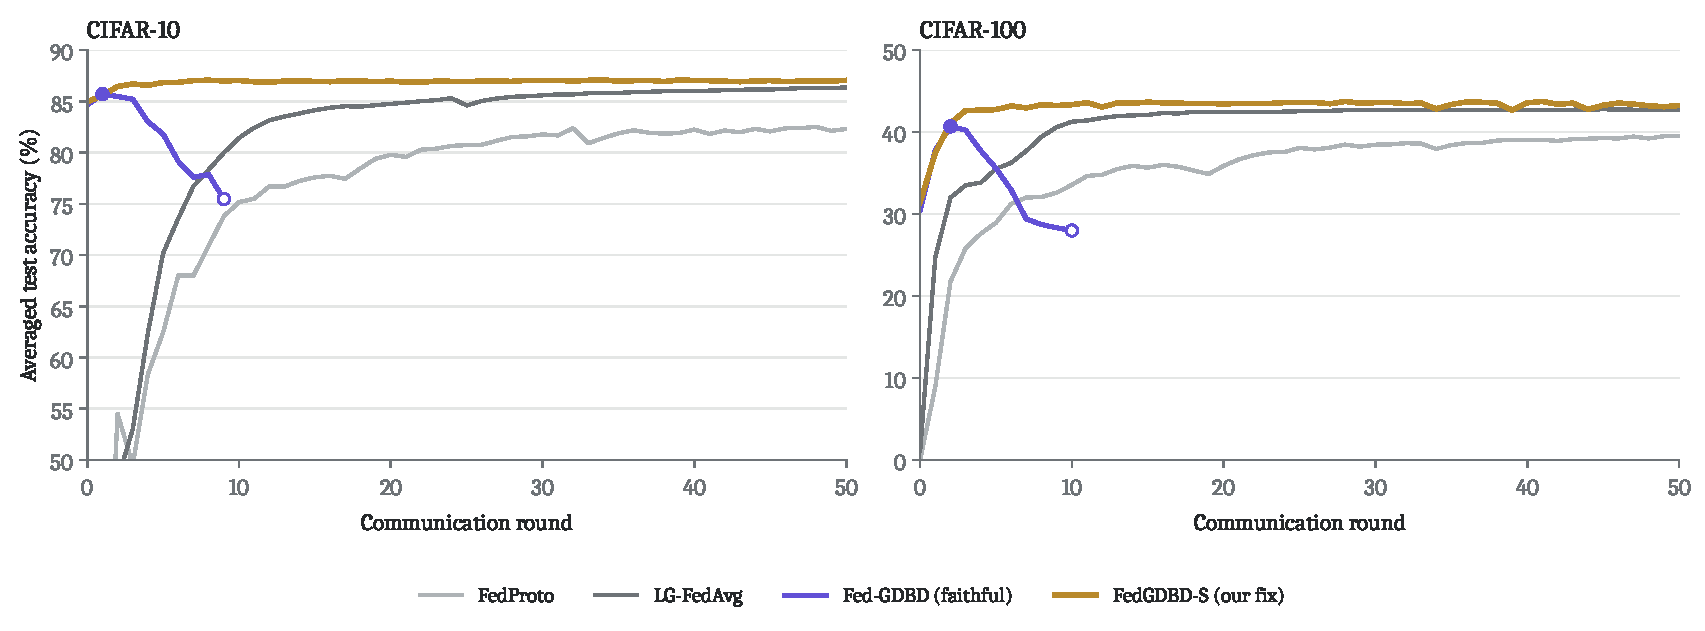
\includegraphics[width=\textwidth]{figures/convergence.pdf}
\caption[Reproduction: accuracy over 50 rounds]{Averaged test accuracy over 50 rounds on CIFAR-10 (left) and CIFAR-100 (right). On the faithful Fed-GDBD line the filled dot marks its best round and the open dot the round at which we stopped it.}
\label{fig:convergence}
\end{figure}

\section{Reproduction: the collapse of the literal update}
\label{sec:res-collapse}

Breaking the accuracy down by architecture shows where the faithful update fails. Table~\ref{tab:collapse} lists the mean accuracy of the five clients of each architecture at the faithful run's best round, at its last round, and for FedGDBD-S at round 50; Figure~\ref{fig:collapse} plots the same numbers.

On CIFAR-100 (Figure~\ref{fig:collapse}b), the CNN clients fall from 48.0\% at round 2 to 3.9\% at round 10, and the ResNet18 clients from 35.7\% to 25.4\%, while GoogLeNet and MobileNetV2 clients keep improving (43.6 to 46.9\% and 35.3 to 36.5\%). On CIFAR-10 (Figure~\ref{fig:collapse}a) the ResNet18 clients suffer most, from 78.7\% to 53.3\%; CNN and GoogLeNet clients lose about 8 pt each and MobileNetV2 clients gain 2.3 pt. The damage is therefore uneven across architectures and different on the two datasets, which is what led us to suspect a mismatch between $g$ and particular feature spaces (Section~\ref{sec:m-fix}). With the fix, every architecture ends at or above the faithful run's best: CIFAR-100 CNN clients recover to 45.6\% and CIFAR-10 ResNet18 clients to 79.2\%.

\begin{table}[htbp]
\centering
\caption[Accuracy per architecture before and after the collapse]{Mean test accuracy (\%) of the five clients of each architecture: faithful Fed-GDBD at its best and last rounds, and FedGDBD-S at round 50.}
\label{tab:collapse}
\small
\TabCollapse
\end{table}

\begin{figure}[htbp]
\centering
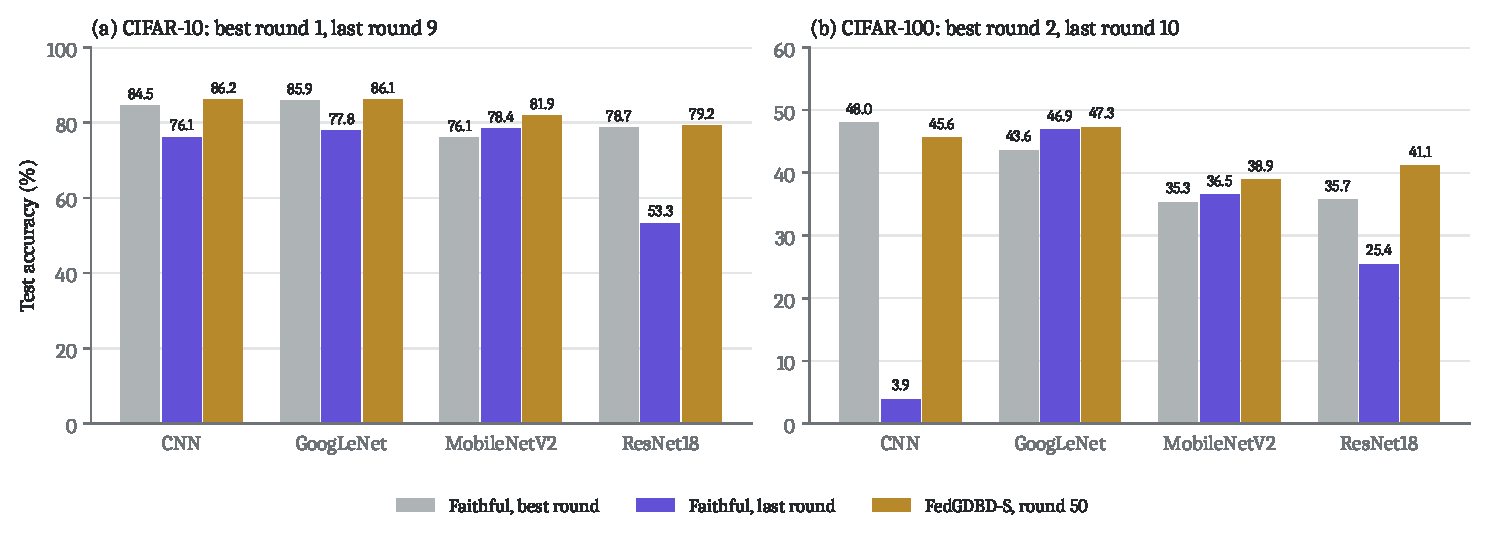
\includegraphics[width=\textwidth]{figures/collapse_both.pdf}
\caption[Collapse of the literal update per architecture]{Accuracy per client architecture for the faithful Fed-GDBD at its best and last rounds, and for FedGDBD-S at round 50. (a) CIFAR-10: the ResNet18 clients fall from 78.7\% to 53.3\% and reach 79.2\% with FedGDBD-S. (b) CIFAR-100: the CNN clients collapse from 48.0\% to 3.9\% and recover to 45.6\%.}
\label{fig:collapse}
\end{figure}

Figure~\ref{fig:ikdbug} answers a natural question: was the collapse caused by our earlier IKD bug (Section~\ref{sec:i-bug})? It was not. The buggy run on CIFAR-100 (grey) peaks at round 2 (41.36\%), declines, and crashes with a NaN loss at round 8. After the fix (purple) the loss stays finite, but the accuracy follows almost the same decline. The bug added a crash; the decline comes from the update in Eq.~\eqref{eq:update}. On CIFAR-10 the buggy run had not diverged when we stopped it after 7 rounds (best 86.82\%, last 84.69\%).

\begin{figure}[htbp]
\centering
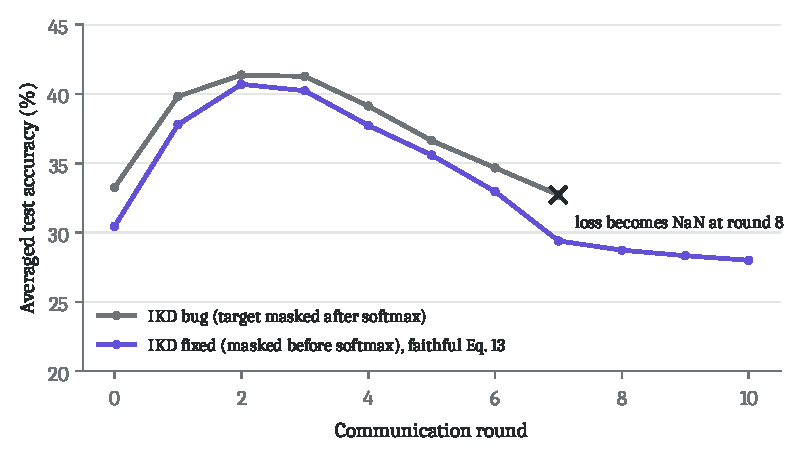
\includegraphics[width=0.72\textwidth]{figures/ikd_bug.pdf}
\caption[Buggy vs fixed IKD loss, CIFAR-100]{CIFAR-100, faithful Fed-GDBD with our first, buggy IKD loss and with the fixed loss. Both decline after round 2; only the buggy one crashes.}
\label{fig:ikdbug}
\end{figure}

\section{Reproduction: per-architecture accuracy of all methods}
\label{sec:res-arch}

Table~\ref{tab:archmethods} and Figure~\ref{fig:archmethods} compare all four methods per architecture at their best rounds. The methods favour different architectures. FedProto is the strongest method on the CNN clients (87.1\% on CIFAR-10, 51.4\% on CIFAR-100) but the weakest on MobileNetV2 (68.6\% and 29.7\%), which suggests that pulling features toward one global mean per class suits some feature extractors far better than others. LG-FedAvg is best on the CIFAR-100 ResNet18 clients (44.3\%). FedGDBD-S is the best on MobileNetV2 on both datasets (81.6\% and 38.8\%) and on GoogLeNet on CIFAR-100 (47.3\%). MobileNetV2 is the hardest architecture for every method.

\begin{table}[htbp]
\centering
\caption[Per-architecture accuracy of all methods]{Mean test accuracy (\%) per client architecture for each method at its best round.}
\label{tab:archmethods}
\small
\TabArchMethods
\end{table}

\begin{figure}[htbp]
\centering
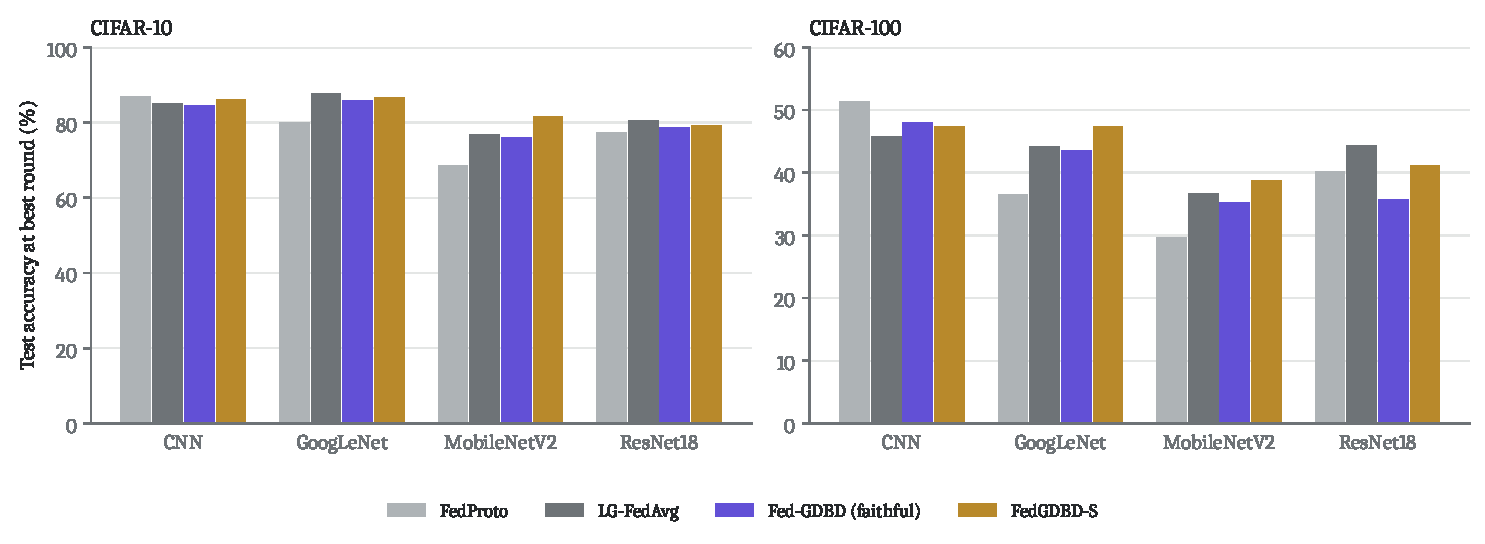
\includegraphics[width=\textwidth]{figures/per_arch_methods.pdf}
\caption[Per-architecture accuracy of all methods]{Accuracy per client architecture for the four methods at their best rounds, CIFAR-10 (left) and CIFAR-100 (right).}
\label{fig:archmethods}
\end{figure}

\section{Reproduction: stability of FedGDBD-S}
\label{sec:res-stab}

FedGDBD-S shows no downward trend over 50 rounds (Figure~\ref{fig:convergence}). From round 3 onward its accuracy never drops more than 0.53 pt below its best on CIFAR-10 and 1.1 pt on CIFAR-100; the larger dips on CIFAR-100 are single rounds (for example 42.70\% at round 39) followed by recovery. Its best rounds were 34 and 28, and its last-round accuracies 87.06\% and 43.25\%.

\section{Extension: agreement-gated distillation}
\label{sec:res-nov}

Table~\ref{tab:novbest} gives the best-round accuracy of the control (FedGDBD-S) and of the two gates for both seeds, with two-seed means and the gap to the control. Figure~\ref{fig:novconv} shows the accuracy curves of all twelve runs.

\begin{table}[htbp]
\centering
\caption[Extension: best-round accuracy]{Extension runs: best-round averaged test accuracy (\%), 20 rounds, validation-slice teacher. The gap is the difference of two-seed means to the control.}
\label{tab:novbest}
\small
\TabNovBest
\end{table}

The per-seed gaps to the control are:
\begin{itemize}
\item AGC on CIFAR-100: $+0.86$ and $+0.52$ (mean $+0.69$).
\item AGS on CIFAR-10: $+0.40$ and $+0.37$ (mean $+0.39$).
\item AGC on CIFAR-10: $-0.04$ and $+0.45$ (mean $+0.21$).
\item AGS on CIFAR-100: $+0.17$ and $-0.14$ (mean $+0.02$).
\end{itemize}
Measured against the criterion fixed before the runs (at least $+0.5$ pt on both datasets), neither gate is an improvement, and we do not claim a general gain. Two results do repeat across both seeds: AGC helps on CIFAR-100 and AGS helps on CIFAR-10. In both cases the gain in each seed is larger than the control's own change between seeds (0.19 and 0.23 pt). With two seeds this is evidence, not proof.

\begin{figure}[htbp]
\centering
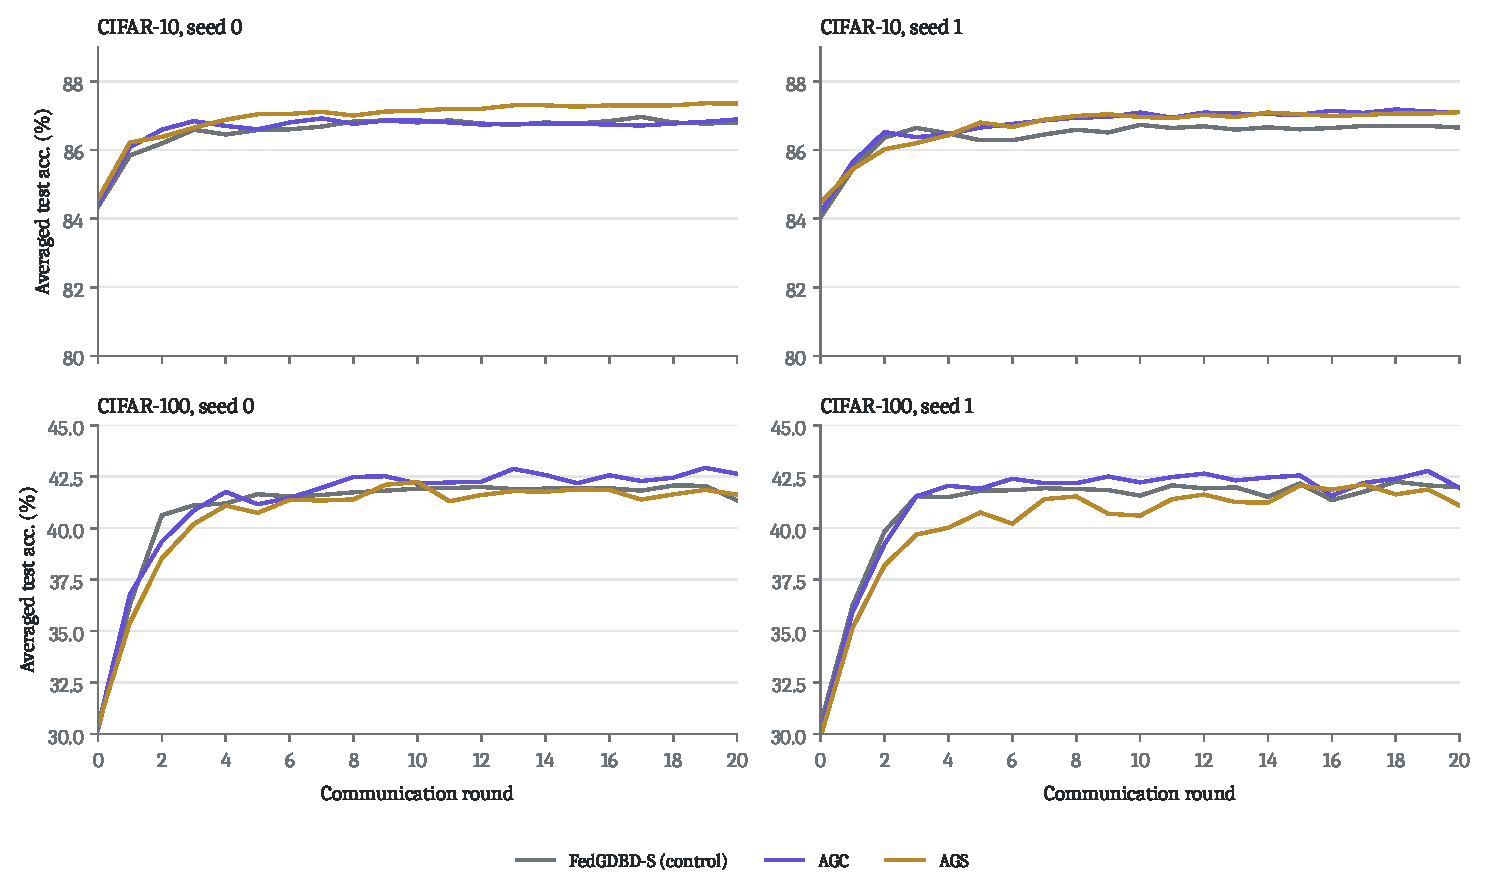
\includegraphics[width=\textwidth]{figures/novelty_convergence.pdf}
\caption[Extension: accuracy over 20 rounds]{Averaged test accuracy over 20 rounds for the control and the two gates, by dataset (rows) and seed (columns).}
\label{fig:novconv}
\end{figure}

The curves in Figure~\ref{fig:novconv} show the same picture over the whole run rather than only at the best round. On CIFAR-10, AGS is above the control in every round of seed 0 and in every round from round 5 of seed 1. On CIFAR-100, AGC is above the control in almost every round after the first few, in both seeds, while AGS stays below it in most rounds: in its first rounds it discards almost all MobileNetV2 images (Section~\ref{sec:res-gate}).

Because best-round reporting is slightly optimistic, Table~\ref{tab:novlast} repeats the comparison at the last round. The conclusions do not change: AGC is $+0.63$ pt above the control on CIFAR-100 and AGS $+0.50$ pt on CIFAR-10, while AGS on CIFAR-100 is now 0.30 pt below.

\begin{table}[htbp]
\centering
\caption[Extension: last-round accuracy]{Extension runs: last-round (round 20) averaged test accuracy (\%).}
\label{tab:novlast}
\small
\TabNovLast
\end{table}

Table~\ref{tab:novarch} lists per-architecture accuracy at the best round for every extension run, and Table~\ref{tab:archgain} with Figure~\ref{fig:archgain} the two-seed mean gain of each gate over the control per architecture. On CIFAR-10 the MobileNetV2 clients gain the most under both gates ($+0.95$ with AGC, $+1.13$ with AGS). On CIFAR-100, AGC helps ResNet18 ($+1.33$) and MobileNetV2 ($+0.87$) most, and AGS costs the CNN clients 0.91 pt, which explains why AGS does not help there overall.

\begin{table}[htbp]
\centering
\caption[Extension: per-architecture accuracy, every run]{Extension runs: mean test accuracy (\%) per client architecture at each run's best round.}
\label{tab:novarch}
\scriptsize
\setlength{\tabcolsep}{4pt}
\TabNovArch
\end{table}

\begin{table}[htbp]
\centering
\caption[Extension: per-architecture gain over the control]{Gain of each gate over the control per architecture (pt), mean of the two seeds, at the best round.}
\label{tab:archgain}
\small
\TabArchGain
\end{table}

\begin{figure}[htbp]
\centering
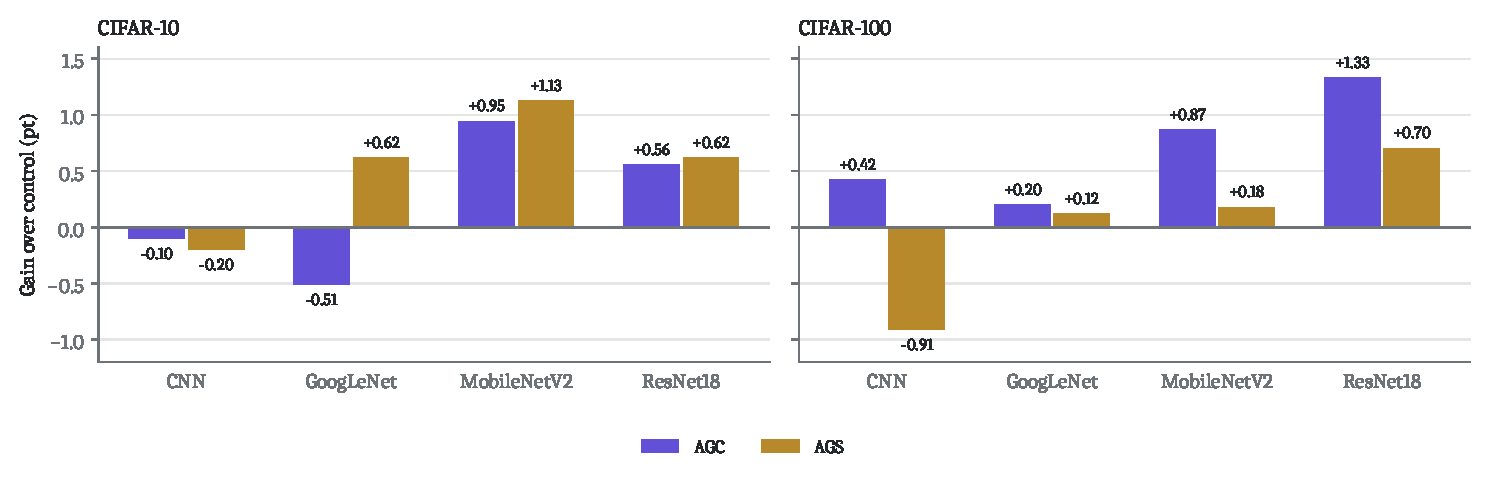
\includegraphics[width=\textwidth]{figures/arch_gains.pdf}
\caption[Extension: per-architecture gain over the control]{Per-architecture gain of AGC and AGS over the control, two-seed means, CIFAR-10 (left) and CIFAR-100 (right).}
\label{fig:archgain}
\end{figure}

\section{Extension: what the gates measured}
\label{sec:res-gate}

The gate statistics in the logs describe how well $g$ fits each architecture. Table~\ref{tab:gate} summarises them, and Figures~\ref{fig:gacc} and~\ref{fig:kept} show how they change over the rounds.

\begin{table}[htbp]
\centering
\caption[Gate statistics per architecture]{Gate statistics per architecture, seed 0 / seed 1. AGC rows: share of the clients' training images that $g$ classifies correctly (the value that scales $\alpha$). AGS rows: share of images actually distilled.}
\label{tab:gate}
\scriptsize
\setlength{\tabcolsep}{4pt}
\TabGate
\end{table}

Measured by AGC, $g$ classifies 96 to 97\% of the CNN clients' CIFAR-10 training images correctly over the run, but only 49 to 53\% of the MobileNetV2 clients'. On CIFAR-100 the figures are 75 to 81\% for CNN, GoogLeNet and ResNet18 against 42 to 44\% for MobileNetV2. At round 0 the gap is extreme: $g$ is right on 11 to 14\% of MobileNetV2 images on CIFAR-10 and 2 to 3\% on CIFAR-100. The gate was never told about architectures, yet in all four runs it singles out MobileNetV2 as the architecture $g$ serves worst.

\begin{figure}[htbp]
\centering
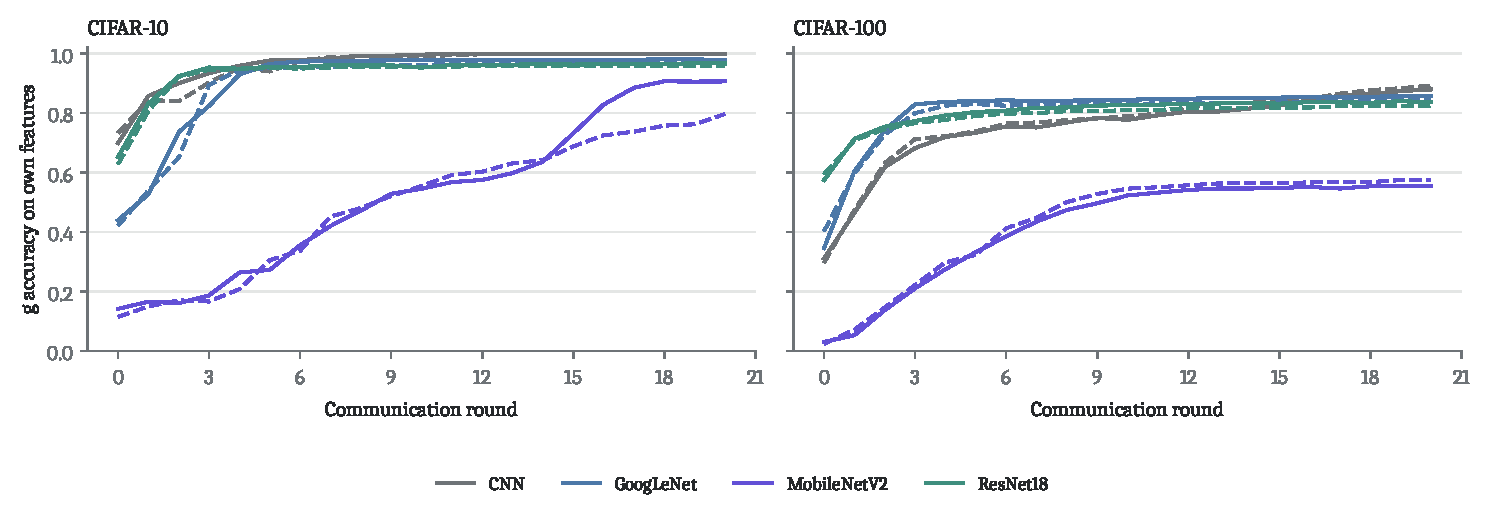
\includegraphics[width=\textwidth]{figures/gate_gacc.pdf}
\caption[AGC: accuracy of $g$ per architecture over rounds]{AGC: accuracy of $g$ on each architecture's own training features over the rounds (solid: seed 0, dashed: seed 1). MobileNetV2 starts far below the others and catches up only partly.}
\label{fig:gacc}
\end{figure}

Figure~\ref{fig:gacc} shows that $g$'s accuracy on MobileNetV2 features rises over the run as $g$ and the clients adapt, to about 0.8 to 0.9 on CIFAR-10 by round 20 and about 0.56 on CIFAR-100, while the other architectures pass 0.7 within about five rounds. So the gate reduces MobileNetV2's distillation weight most in the early rounds and less later.

\begin{figure}[htbp]
\centering
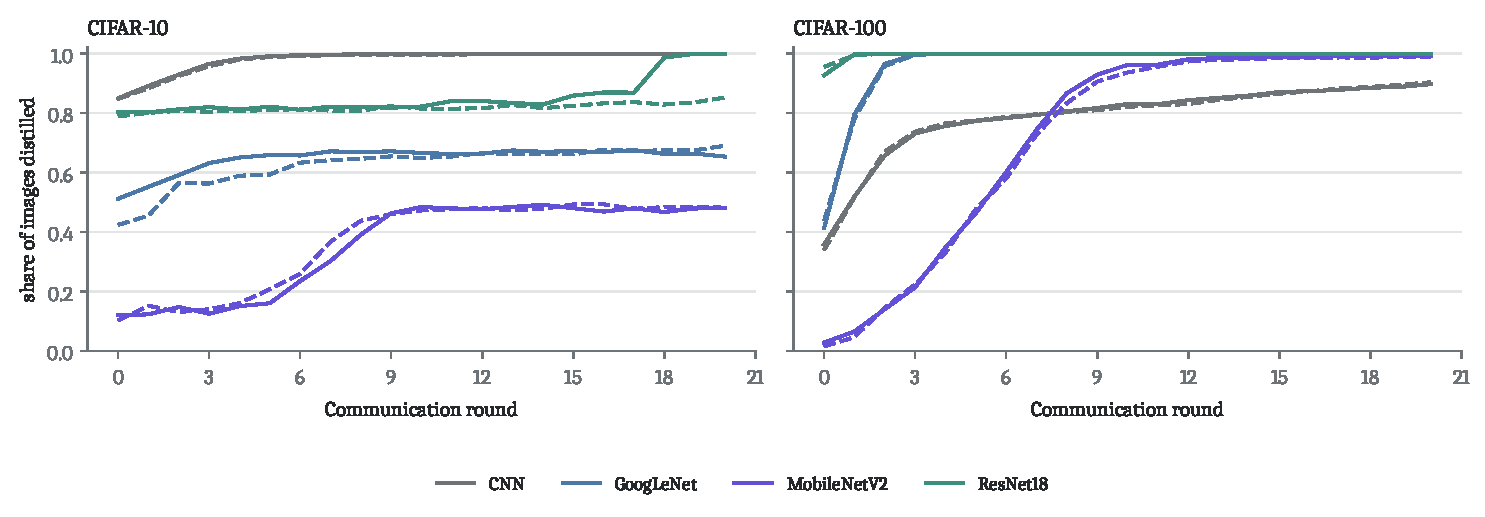
\includegraphics[width=\textwidth]{figures/gate_kept.pdf}
\caption[AGS: share of images distilled over rounds]{AGS: share of each architecture's images that were distilled in each round (solid: seed 0, dashed: seed 1).}
\label{fig:kept}
\end{figure}

AGS (Figure~\ref{fig:kept}) shows the same pattern from a different angle. On CIFAR-10, MobileNetV2 clients distil only 36 to 37\% of their images on average and GoogLeNet clients 62 to 65\%, while CNN clients distil 98\%. On CIFAR-100 nearly all images of the GoogLeNet and ResNet18 clients are distilled after a few rounds, MobileNetV2 climbs from 1 to 3\% at round 0 to almost all, and the CNN clients rise slowly from about 35\% to about 90\%. These kept fractions are counted during training (model in training mode), so they differ from AGC's evaluation-mode accuracy, but both point to MobileNetV2.

\section{Discussion}
\label{sec:discussion}

\textbf{Why the literal update collapses.} The collapse hits different architectures on the two datasets and builds up over several rounds. Both facts fit our explanation: a scale mismatch between $g$'s logits and some clients' heads, amplified by the KD weight $\alpha T^2 = 280$, so that distillation overrides cross-entropy and reshapes the extractor. The fix works by removing exactly these two channels (the scale and the gradient into the extractor), which supports the explanation, but we did not log logit norms to confirm it directly. The authors' unreleased code may include a detail that avoids the problem, such as a normalisation or a smaller learning rate.

\textbf{Why each gate helps a different dataset.} This is our interpretation and not proven. On CIFAR-100, $g$ is wrong often, but its softened predictions still carry information about which of the 100 classes look alike, so turning the distillation down smoothly (AGC) keeps that information while reducing the harm. Discarding images (AGS) throws it away, and in the first rounds AGS discards almost all MobileNetV2 images. On CIFAR-10, $g$ is right on most images and there are only 10 classes, so removing only the images $g$ gets wrong (AGS) cleans up the signal without losing much.

\textbf{The architecture finding.} The clearest result of the extension is not an accuracy gain but a measurement: one linear boundary shared by four architectures fits them very unequally, and the unevenness is large (about 0.5 vs 0.97 on CIFAR-10). It matches what the baselines show in Table~\ref{tab:archmethods}, where MobileNetV2 is the hardest architecture for every method and FedProto, which also imposes one global target per class, is weakest exactly there. The gains follow the measurement on CIFAR-10, where MobileNetV2 benefits most; on CIFAR-100 the largest AGC gain goes to ResNet18, so the link is not one-to-one.

\textbf{Threats to validity.} Two seeds cannot give a reliable estimate of a 0.4 pt effect. All accuracies are best-round values, as in the paper, which is optimistic; the last-round results agree, which reduces this concern. In the reproduction the IKD teacher was picked by test accuracy, a mild use of test data shared by Fed-GDBD and FedGDBD-S; the extension runs avoid it. GPU nondeterminism and the unseeded client order in the reproduction runs mean a rerun will differ slightly.

\section{Limitations}

\begin{table}[htbp]
\centering
\caption[Limitations and remedies]{Limitations of this study and what would address them.}
\label{tab:limits}
\small
\begin{tabularx}{\textwidth}{>{\raggedright\arraybackslash}X>{\raggedright\arraybackslash}p{3.4cm}>{\raggedright\arraybackslash}X}
\toprule
Limitation & Reason & Remedy \\
\midrule
Two of the paper's four datasets; practical split only & compute & Tiny-ImageNet, Flowers102, pathological split \\
Reproduction: 50 rounds, one run (paper: 100 $\times$ 3) & compute & full-length runs with three seeds \\
Extension: two seeds, 20 rounds & compute & five or more seeds, reported as mean $\pm$ SD \\
Collapse explanation not proven & no logit statistics logged & log logit scales per architecture \\
No ablation of $\alpha$, $T$, or a fixed smaller $\alpha$ for all clients & time & run these as additional controls \\
Only FedProto and LG-FedAvg as baselines & compute & add FedTGP and FedGH (already in HtFLlib) \\
\bottomrule
\end{tabularx}
\end{table}

Table~\ref{tab:limits} lists the main limitations. The missing control for AGC deserves a note: AGC lowers the distillation weight only for clients $g$ misreads, and well-served clients keep almost the paper's value, so it is not the same as lowering $\alpha$ for everyone. But we did not run that comparison, and it is the first one a sceptical reader would ask for.

\section{Future work}

\begin{enumerate}
\item Repeat the extension with five or more seeds and report mean $\pm$ standard deviation, so that effects of a few tenths of a point can be measured properly.
\item Run 50 to 100 rounds, the paper's other datasets and the pathological split.
\item Add the missing controls: a sweep over $\alpha$ and $T$ and a run with one smaller $\alpha$ for all clients.
\item Try a soft gate, using $g$'s probability for the true label as the weight instead of a 0/1 decision, and a hybrid that uses AGC where $\mathrm{acc}_i$ is low and AGS where it is high.
\item Test the collapse explanation directly by logging the logit scales of $g$ and of each head per architecture.
\end{enumerate}

\section{Conclusion}

We re-implemented Fed-GDBD from its paper and reproduced its main experiment on CIFAR-10 and CIFAR-100. The baselines matched the published numbers closely, which gives confidence in the setup. The literal client update turned out to be unstable for particular architectures; two changes to the distillation step, logit-scale matching and head-only distillation, fixed it without touching the paper's hyper-parameters, and the fixed version was the best method in our runs, about one point below the paper's reported results with half the training.

Our extension gates the distillation of the global boundary by whether it agrees with each client's labels. It gave gains that repeated across two seeds on one dataset each (AGC on CIFAR-100, AGS on CIFAR-10), but it did not meet the bar we set in advance, and we do not claim that it improves Fed-GDBD in general. Its main lasting result is the measurement behind it: a single global boundary fits some client architectures far worse than others, and a client can detect this from its own data at no communication cost. Measuring that properly, with more seeds and the missing controls, is the natural next step.


\clearpage
\addcontentsline{toc}{chapter}{REFERENCES}
\begin{thebibliography}{99}
\setlength{\itemsep}{0.25em}

\bibitem{zhang2025gdbd}
K.~Zhang, J.~Wang, W.~Wang, T.~Zeng, P.~Li, X.~Wang, and T.~Zhang, ``Federated learning with heterogeneous data and models based on global decision boundary distillation,'' \emph{Journal of King Saud University -- Computer and Information Sciences}, vol.~37, art.~75, 2025, doi:10.1007/s44443-025-00097-0.

\bibitem{mcmahan2017fedavg}
B.~McMahan, E.~Moore, D.~Ramage, S.~Hampson, and B.~Ag\"{u}era y Arcas, ``Communication-efficient learning of deep networks from decentralized data,'' in \emph{Proc. Int. Conf. Artificial Intelligence and Statistics (AISTATS)}, 2017, pp.~1273--1282.

\bibitem{hsu2019noniid}
T.-M.~H.~Hsu, H.~Qi, and M.~Brown, ``Measuring the effects of non-identical data distribution for federated visual classification,'' arXiv:1909.06335, 2019.

\bibitem{liang2020lgfedavg}
P.~P.~Liang, T.~Liu, L.~Ziyin, N.~B.~Allen, R.~P.~Auerbach, D.~Brent, R.~Salakhutdinov, and L.-P.~Morency, ``Think locally, act globally: Federated learning with local and global representations,'' arXiv:2001.01523, 2020.

\bibitem{tan2022fedproto}
Y.~Tan, G.~Long, L.~Liu, T.~Zhou, Q.~Lu, J.~Jiang, and C.~Zhang, ``FedProto: Federated prototype learning across heterogeneous clients,'' in \emph{Proc. AAAI Conf. Artificial Intelligence}, 2022.

\bibitem{zhang2024fedtgp}
J.~Zhang, Y.~Liu, Y.~Hua, and J.~Cao, ``FedTGP: Trainable global prototypes with adaptive-margin-enhanced contrastive learning for data and model heterogeneity in federated learning,'' in \emph{Proc. AAAI Conf. Artificial Intelligence}, vol.~38, 2024.

\bibitem{yi2023fedgh}
L.~Yi, G.~Wang, X.~Liu, Z.~Shi, and H.~Yu, ``FedGH: Heterogeneous federated learning with generalized global header,'' in \emph{Proc. ACM Int. Conf. Multimedia (MM)}, 2023.

\bibitem{zhang2025htfllib}
J.~Zhang \emph{et al.}, ``HtFLlib: A comprehensive heterogeneous federated learning library and benchmark,'' in \emph{Proc. ACM SIGKDD Conf. Knowledge Discovery and Data Mining}, 2025.

\bibitem{zhang2025pfllib}
J.~Zhang \emph{et al.}, ``PFLlib: A beginner-friendly and comprehensive personalized federated learning library and benchmark,'' \emph{Journal of Machine Learning Research}, vol.~26, 2025.

\bibitem{hinton2015kd}
G.~Hinton, O.~Vinyals, and J.~Dean, ``Distilling the knowledge in a neural network,'' arXiv:1503.02531, 2015.

\bibitem{zhao2022dkd}
B.~Zhao, Q.~Cui, R.~Song, Y.~Qiu, and J.~Liang, ``Decoupled knowledge distillation,'' in \emph{Proc. IEEE/CVF Conf. Computer Vision and Pattern Recognition (CVPR)}, 2022.

\bibitem{arthur2007kmeanspp}
D.~Arthur and S.~Vassilvitskii, ``k-means++: The advantages of careful seeding,'' in \emph{Proc. ACM-SIAM Symp. Discrete Algorithms (SODA)}, 2007, pp.~1027--1035.

\bibitem{krizhevsky2009cifar}
A.~Krizhevsky, ``Learning multiple layers of features from tiny images,'' Technical report, University of Toronto, 2009.

\bibitem{szegedy2015googlenet}
C.~Szegedy \emph{et al.}, ``Going deeper with convolutions,'' in \emph{Proc. IEEE Conf. Computer Vision and Pattern Recognition (CVPR)}, 2015.

\bibitem{sandler2018mobilenetv2}
M.~Sandler, A.~Howard, M.~Zhu, A.~Zhmoginov, and L.-C.~Chen, ``MobileNetV2: Inverted residuals and linear bottlenecks,'' in \emph{Proc. IEEE/CVF Conf. Computer Vision and Pattern Recognition (CVPR)}, 2018.

\bibitem{he2016resnet}
K.~He, X.~Zhang, S.~Ren, and J.~Sun, ``Deep residual learning for image recognition,'' in \emph{Proc. IEEE Conf. Computer Vision and Pattern Recognition (CVPR)}, 2016.

\end{thebibliography}


\appendix
\chapter{Reproducing the Results}
\label{app:repro}

The repository is \url{https://github.com/md25052007/Fed-GDBD-for-HtFL}; its \texttt{REPRODUCTION.md} gives these steps in more detail, with troubleshooting. All commands run from the repository folder on Windows.

\begin{enumerate}
\item \textbf{Set up.} \texttt{setup.bat} creates a virtual environment and installs PyTorch with CUDA and the requirements.
\item \textbf{Data.} The launchers download CIFAR-10 and CIFAR-100 and build the split (\texttt{python generate\_Cifar10.py noniid - dir} in \texttt{dataset/}). If the download stalls, place \texttt{cifar-10-python.tar.gz} or \texttt{cifar-100-python.tar.gz} in \texttt{dataset/Cifar10/rawdata/} or \texttt{dataset/Cifar100/rawdata/}.
\item \textbf{Reproduction runs.} \texttt{run\_cifar10.bat} and \texttt{run\_cifar100.bat} start the faithful Fed-GDBD, FedProto and LG-FedAvg; \texttt{start\_fedgdbd\_s\_cifar10.bat} and \texttt{start\_fedgdbd\_s\_cifar100.bat} start FedGDBD-S. Each run executes
\begin{quote}\small\ttfamily
python main.py -data Cifar10 -ncl 10 -m HtFE-img-4 -fd 512 -nc 20 -jr 1 -lbs 10 -lr 0.01 -ls 5 -gr 50 -t 1 -go practical -did 0 -algo FedGDBD-S
\end{quote}
with \texttt{-algo} set to \texttt{FedGDBD}, \texttt{FedGDBD-S}, \texttt{FedProto} (with \texttt{-lam 10}) or \texttt{LG-FedAvg}.
\item \textbf{Extension runs.} \texttt{run\_novelty\_cifar10.bat} and \texttt{run\_novelty\_cifar100.bat} (seed 0), \texttt{run\_novelty\_cifar10\_seed1.bat} and \texttt{run\_novelty\_cifar100\_seed1.bat} (seed 1) start the control, AGC and AGS with \texttt{-gr 20 --gdbd\_teacher val --seed} $s$.
\item \textbf{Tables and figures.} From the saved logs, without training:
\begin{quote}\small\ttfamily
python progress.py experiments\textbackslash cifar10\textbackslash logs\\
python analysis\textbackslash novelty\_summary.py experiments\textbackslash novelty\textbackslash run2\_seed1\textbackslash cifar100\textbackslash logs\\
python analysis\textbackslash report\_assets.py\\
python analysis\textbackslash report\_tables.py
\end{quote}
The last two regenerate every figure and results table of Chapter~\ref{ch:results}.
\end{enumerate}

\chapter{Per-client Results}
\label{app:clients}

Tables~\ref{tab:clients10} and~\ref{tab:clients100} give each client's test accuracy at the best round of each reproduction run. They show how much the clients differ under the skewed split, and where the per-architecture means in Table~\ref{tab:archmethods} come from.

\vspace{0.8em}
\noindent\begin{minipage}{\textwidth}
\begin{spacing}{1.0}\centering
\captionof{table}[Per-client accuracy, CIFAR-10]{CIFAR-10: test accuracy (\%) of each client at the best round of each reproduction run.}
\label{tab:clients10}
\footnotesize
\renewcommand{\arraystretch}{0.9}
\TabClientsTen

\vspace{1.0em}
\captionof{table}[Per-client accuracy, CIFAR-100]{CIFAR-100: test accuracy (\%) of each client at the best round of each reproduction run.}
\label{tab:clients100}
\TabClientsHundred
\end{spacing}
\end{minipage}


\end{document}
